% Options for packages loaded elsewhere
\PassOptionsToPackage{unicode}{hyperref}
\PassOptionsToPackage{hyphens}{url}
\PassOptionsToPackage{dvipsnames,svgnames,x11names}{xcolor}
%
\documentclass[
  letterpaper,
  DIV=11,
  numbers=noendperiod]{scrartcl}

\usepackage{amsmath,amssymb}
\usepackage{iftex}
\ifPDFTeX
  \usepackage[T1]{fontenc}
  \usepackage[utf8]{inputenc}
  \usepackage{textcomp} % provide euro and other symbols
\else % if luatex or xetex
  \usepackage{unicode-math}
  \defaultfontfeatures{Scale=MatchLowercase}
  \defaultfontfeatures[\rmfamily]{Ligatures=TeX,Scale=1}
\fi
\usepackage{lmodern}
\ifPDFTeX\else  
    % xetex/luatex font selection
\fi
% Use upquote if available, for straight quotes in verbatim environments
\IfFileExists{upquote.sty}{\usepackage{upquote}}{}
\IfFileExists{microtype.sty}{% use microtype if available
  \usepackage[]{microtype}
  \UseMicrotypeSet[protrusion]{basicmath} % disable protrusion for tt fonts
}{}
\makeatletter
\@ifundefined{KOMAClassName}{% if non-KOMA class
  \IfFileExists{parskip.sty}{%
    \usepackage{parskip}
  }{% else
    \setlength{\parindent}{0pt}
    \setlength{\parskip}{6pt plus 2pt minus 1pt}}
}{% if KOMA class
  \KOMAoptions{parskip=half}}
\makeatother
\usepackage{xcolor}
\setlength{\emergencystretch}{3em} % prevent overfull lines
\setcounter{secnumdepth}{5}
% Make \paragraph and \subparagraph free-standing
\ifx\paragraph\undefined\else
  \let\oldparagraph\paragraph
  \renewcommand{\paragraph}[1]{\oldparagraph{#1}\mbox{}}
\fi
\ifx\subparagraph\undefined\else
  \let\oldsubparagraph\subparagraph
  \renewcommand{\subparagraph}[1]{\oldsubparagraph{#1}\mbox{}}
\fi

\usepackage{color}
\usepackage{fancyvrb}
\newcommand{\VerbBar}{|}
\newcommand{\VERB}{\Verb[commandchars=\\\{\}]}
\DefineVerbatimEnvironment{Highlighting}{Verbatim}{commandchars=\\\{\}}
% Add ',fontsize=\small' for more characters per line
\usepackage{framed}
\definecolor{shadecolor}{RGB}{241,243,245}
\newenvironment{Shaded}{\begin{snugshade}}{\end{snugshade}}
\newcommand{\AlertTok}[1]{\textcolor[rgb]{0.68,0.00,0.00}{#1}}
\newcommand{\AnnotationTok}[1]{\textcolor[rgb]{0.37,0.37,0.37}{#1}}
\newcommand{\AttributeTok}[1]{\textcolor[rgb]{0.40,0.45,0.13}{#1}}
\newcommand{\BaseNTok}[1]{\textcolor[rgb]{0.68,0.00,0.00}{#1}}
\newcommand{\BuiltInTok}[1]{\textcolor[rgb]{0.00,0.23,0.31}{#1}}
\newcommand{\CharTok}[1]{\textcolor[rgb]{0.13,0.47,0.30}{#1}}
\newcommand{\CommentTok}[1]{\textcolor[rgb]{0.37,0.37,0.37}{#1}}
\newcommand{\CommentVarTok}[1]{\textcolor[rgb]{0.37,0.37,0.37}{\textit{#1}}}
\newcommand{\ConstantTok}[1]{\textcolor[rgb]{0.56,0.35,0.01}{#1}}
\newcommand{\ControlFlowTok}[1]{\textcolor[rgb]{0.00,0.23,0.31}{#1}}
\newcommand{\DataTypeTok}[1]{\textcolor[rgb]{0.68,0.00,0.00}{#1}}
\newcommand{\DecValTok}[1]{\textcolor[rgb]{0.68,0.00,0.00}{#1}}
\newcommand{\DocumentationTok}[1]{\textcolor[rgb]{0.37,0.37,0.37}{\textit{#1}}}
\newcommand{\ErrorTok}[1]{\textcolor[rgb]{0.68,0.00,0.00}{#1}}
\newcommand{\ExtensionTok}[1]{\textcolor[rgb]{0.00,0.23,0.31}{#1}}
\newcommand{\FloatTok}[1]{\textcolor[rgb]{0.68,0.00,0.00}{#1}}
\newcommand{\FunctionTok}[1]{\textcolor[rgb]{0.28,0.35,0.67}{#1}}
\newcommand{\ImportTok}[1]{\textcolor[rgb]{0.00,0.46,0.62}{#1}}
\newcommand{\InformationTok}[1]{\textcolor[rgb]{0.37,0.37,0.37}{#1}}
\newcommand{\KeywordTok}[1]{\textcolor[rgb]{0.00,0.23,0.31}{#1}}
\newcommand{\NormalTok}[1]{\textcolor[rgb]{0.00,0.23,0.31}{#1}}
\newcommand{\OperatorTok}[1]{\textcolor[rgb]{0.37,0.37,0.37}{#1}}
\newcommand{\OtherTok}[1]{\textcolor[rgb]{0.00,0.23,0.31}{#1}}
\newcommand{\PreprocessorTok}[1]{\textcolor[rgb]{0.68,0.00,0.00}{#1}}
\newcommand{\RegionMarkerTok}[1]{\textcolor[rgb]{0.00,0.23,0.31}{#1}}
\newcommand{\SpecialCharTok}[1]{\textcolor[rgb]{0.37,0.37,0.37}{#1}}
\newcommand{\SpecialStringTok}[1]{\textcolor[rgb]{0.13,0.47,0.30}{#1}}
\newcommand{\StringTok}[1]{\textcolor[rgb]{0.13,0.47,0.30}{#1}}
\newcommand{\VariableTok}[1]{\textcolor[rgb]{0.07,0.07,0.07}{#1}}
\newcommand{\VerbatimStringTok}[1]{\textcolor[rgb]{0.13,0.47,0.30}{#1}}
\newcommand{\WarningTok}[1]{\textcolor[rgb]{0.37,0.37,0.37}{\textit{#1}}}

\providecommand{\tightlist}{%
  \setlength{\itemsep}{0pt}\setlength{\parskip}{0pt}}\usepackage{longtable,booktabs,array}
\usepackage{calc} % for calculating minipage widths
% Correct order of tables after \paragraph or \subparagraph
\usepackage{etoolbox}
\makeatletter
\patchcmd\longtable{\par}{\if@noskipsec\mbox{}\fi\par}{}{}
\makeatother
% Allow footnotes in longtable head/foot
\IfFileExists{footnotehyper.sty}{\usepackage{footnotehyper}}{\usepackage{footnote}}
\makesavenoteenv{longtable}
\usepackage{graphicx}
\makeatletter
\def\maxwidth{\ifdim\Gin@nat@width>\linewidth\linewidth\else\Gin@nat@width\fi}
\def\maxheight{\ifdim\Gin@nat@height>\textheight\textheight\else\Gin@nat@height\fi}
\makeatother
% Scale images if necessary, so that they will not overflow the page
% margins by default, and it is still possible to overwrite the defaults
% using explicit options in \includegraphics[width, height, ...]{}
\setkeys{Gin}{width=\maxwidth,height=\maxheight,keepaspectratio}
% Set default figure placement to htbp
\makeatletter
\def\fps@figure{htbp}
\makeatother

\KOMAoption{captions}{tableheading}
\makeatletter
\makeatother
\makeatletter
\makeatother
\makeatletter
\@ifpackageloaded{caption}{}{\usepackage{caption}}
\AtBeginDocument{%
\ifdefined\contentsname
  \renewcommand*\contentsname{Table of contents}
\else
  \newcommand\contentsname{Table of contents}
\fi
\ifdefined\listfigurename
  \renewcommand*\listfigurename{List of Figures}
\else
  \newcommand\listfigurename{List of Figures}
\fi
\ifdefined\listtablename
  \renewcommand*\listtablename{List of Tables}
\else
  \newcommand\listtablename{List of Tables}
\fi
\ifdefined\figurename
  \renewcommand*\figurename{Figure}
\else
  \newcommand\figurename{Figure}
\fi
\ifdefined\tablename
  \renewcommand*\tablename{Table}
\else
  \newcommand\tablename{Table}
\fi
}
\@ifpackageloaded{float}{}{\usepackage{float}}
\floatstyle{ruled}
\@ifundefined{c@chapter}{\newfloat{codelisting}{h}{lop}}{\newfloat{codelisting}{h}{lop}[chapter]}
\floatname{codelisting}{Listing}
\newcommand*\listoflistings{\listof{codelisting}{List of Listings}}
\makeatother
\makeatletter
\@ifpackageloaded{caption}{}{\usepackage{caption}}
\@ifpackageloaded{subcaption}{}{\usepackage{subcaption}}
\makeatother
\makeatletter
\@ifpackageloaded{tcolorbox}{}{\usepackage[skins,breakable]{tcolorbox}}
\makeatother
\makeatletter
\@ifundefined{shadecolor}{\definecolor{shadecolor}{rgb}{.97, .97, .97}}
\makeatother
\makeatletter
\makeatother
\makeatletter
\makeatother
\ifLuaTeX
  \usepackage{selnolig}  % disable illegal ligatures
\fi
\IfFileExists{bookmark.sty}{\usepackage{bookmark}}{\usepackage{hyperref}}
\IfFileExists{xurl.sty}{\usepackage{xurl}}{} % add URL line breaks if available
\urlstyle{same} % disable monospaced font for URLs
\hypersetup{
  pdftitle={Lab\_5\_correlation\_regression\_t\_chi},
  pdfauthor={Justin Baumann},
  colorlinks=true,
  linkcolor={blue},
  filecolor={Maroon},
  citecolor={Blue},
  urlcolor={Blue},
  pdfcreator={LaTeX via pandoc}}

\title{Lab\_5\_correlation\_regression\_t\_chi}
\author{Justin Baumann}
\date{}

\begin{document}
\maketitle
\ifdefined\Shaded\renewenvironment{Shaded}{\begin{tcolorbox}[boxrule=0pt, breakable, borderline west={3pt}{0pt}{shadecolor}, frame hidden, interior hidden, sharp corners, enhanced]}{\end{tcolorbox}}\fi

\renewcommand*\contentsname{Table of contents}
{
\hypersetup{linkcolor=}
\setcounter{tocdepth}{3}
\tableofcontents
}
\hypertarget{learning-objectives}{%
\section{\texorpdfstring{\textbf{Learning
Objectives}}{Learning Objectives}}\label{learning-objectives}}

1.) Explore correlations between numerical variables (two variables and
many)\\
2.) Practice running and interpreting linear regressions\\
3.) Calculate and interpret R\^{}2 values\\
4.) Test assumptions of linear regression\\
5.) practice running and interpreting t-tests\\
6.) test assumptions of t-tests\\
7.) Practice chi-square tests and understand their application\\
\hspace*{0.333em}

\hypertarget{load-packages}{%
\section{\texorpdfstring{\textbf{1: Load
packages}}{1: Load packages}}\label{load-packages}}

\begin{Shaded}
\begin{Highlighting}[]
\FunctionTok{library}\NormalTok{(tidyverse)}
\end{Highlighting}
\end{Shaded}

\begin{verbatim}
Warning: package 'tidyverse' was built under R version 4.2.3
\end{verbatim}

\begin{verbatim}
Warning: package 'ggplot2' was built under R version 4.2.3
\end{verbatim}

\begin{verbatim}
Warning: package 'tibble' was built under R version 4.2.3
\end{verbatim}

\begin{verbatim}
Warning: package 'tidyr' was built under R version 4.2.3
\end{verbatim}

\begin{verbatim}
Warning: package 'readr' was built under R version 4.2.3
\end{verbatim}

\begin{verbatim}
Warning: package 'purrr' was built under R version 4.2.3
\end{verbatim}

\begin{verbatim}
Warning: package 'dplyr' was built under R version 4.2.3
\end{verbatim}

\begin{verbatim}
Warning: package 'forcats' was built under R version 4.2.3
\end{verbatim}

\begin{verbatim}
Warning: package 'lubridate' was built under R version 4.2.3
\end{verbatim}

\begin{verbatim}
-- Attaching core tidyverse packages ------------------------ tidyverse 2.0.0 --
v dplyr     1.1.2     v readr     2.1.4
v forcats   1.0.0     v stringr   1.5.0
v ggplot2   3.4.2     v tibble    3.2.1
v lubridate 1.9.2     v tidyr     1.3.0
v purrr     1.0.1     
-- Conflicts ------------------------------------------ tidyverse_conflicts() --
x dplyr::filter() masks stats::filter()
x dplyr::lag()    masks stats::lag()
i Use the conflicted package (<http://conflicted.r-lib.org/>) to force all conflicts to become errors
\end{verbatim}

\begin{Shaded}
\begin{Highlighting}[]
\FunctionTok{library}\NormalTok{(see)}
\end{Highlighting}
\end{Shaded}

\begin{verbatim}
Warning: package 'see' was built under R version 4.2.3
\end{verbatim}

\begin{Shaded}
\begin{Highlighting}[]
\FunctionTok{library}\NormalTok{(car)}
\end{Highlighting}
\end{Shaded}

\begin{verbatim}
Warning: package 'car' was built under R version 4.2.3
\end{verbatim}

\begin{verbatim}
Loading required package: carData

Attaching package: 'car'

The following object is masked from 'package:dplyr':

    recode

The following object is masked from 'package:purrr':

    some
\end{verbatim}

\begin{Shaded}
\begin{Highlighting}[]
\FunctionTok{library}\NormalTok{(patchwork)}
\FunctionTok{library}\NormalTok{(ggsci)}
\end{Highlighting}
\end{Shaded}

\begin{verbatim}
Warning: package 'ggsci' was built under R version 4.2.3
\end{verbatim}

\begin{verbatim}

Attaching package: 'ggsci'

The following objects are masked from 'package:see':

    scale_color_material, scale_colour_material, scale_fill_material
\end{verbatim}

\begin{Shaded}
\begin{Highlighting}[]
\FunctionTok{library}\NormalTok{(ggridges)}
\FunctionTok{library}\NormalTok{(performance)}
\end{Highlighting}
\end{Shaded}

\begin{verbatim}
Warning: package 'performance' was built under R version 4.2.3
\end{verbatim}

\begin{Shaded}
\begin{Highlighting}[]
\FunctionTok{library}\NormalTok{(Hmisc) }\CommentTok{\#for correlation matrix}
\end{Highlighting}
\end{Shaded}

\begin{verbatim}
Warning: package 'Hmisc' was built under R version 4.2.3
\end{verbatim}

\begin{verbatim}

Attaching package: 'Hmisc'

The following objects are masked from 'package:dplyr':

    src, summarize

The following objects are masked from 'package:base':

    format.pval, units
\end{verbatim}

\begin{Shaded}
\begin{Highlighting}[]
\FunctionTok{library}\NormalTok{(corrplot)}\CommentTok{\#to visualize correlation matrices}
\end{Highlighting}
\end{Shaded}

\begin{verbatim}
Warning: package 'corrplot' was built under R version 4.2.3
\end{verbatim}

\begin{verbatim}
corrplot 0.92 loaded
\end{verbatim}

\begin{Shaded}
\begin{Highlighting}[]
\FunctionTok{library}\NormalTok{(car) }\CommentTok{\#contains some statistical tests we need to assess assumptions}
\end{Highlighting}
\end{Shaded}

\hypertarget{correlation-between-numerical-variables}{%
\section{\texorpdfstring{\textbf{2: Correlation between numerical
variables}}{2: Correlation between numerical variables}}\label{correlation-between-numerical-variables}}

\subsection{Correlation Coefficients}

A \textbf{correlation coefficient (r)} tells us the relationship
(strength and direction) between two variables. These coefficients can
be positive or negative and will range from 0 to 1 (or negative 1).
Values nearer to 1 (or negative 1) indicate stronger correlations and
values closer to 0 indicate weaker correlations

Let's try out some correlations using the iris data.\\
Is there a correlation between sepal length and sepal width? Let's test
each species separately for now.\\
\textbf{Step 1: make a scatterplot}

\begin{Shaded}
\begin{Highlighting}[]
\CommentTok{\#filter down to a single species}
\NormalTok{virg}\OtherTok{\textless{}{-}}\NormalTok{iris }\SpecialCharTok{\%\textgreater{}\%}
  \FunctionTok{filter}\NormalTok{(Species}\SpecialCharTok{==}\StringTok{\textquotesingle{}virginica\textquotesingle{}}\NormalTok{)}

\CommentTok{\#make a plot}
\FunctionTok{ggplot}\NormalTok{(virg, }\FunctionTok{aes}\NormalTok{(}\AttributeTok{x=}\NormalTok{Sepal.Length, }\AttributeTok{y=}\NormalTok{Sepal.Width))}\SpecialCharTok{+}
  \FunctionTok{geom\_point}\NormalTok{()}\SpecialCharTok{+}
  \FunctionTok{theme\_classic}\NormalTok{()}
\end{Highlighting}
\end{Shaded}

\begin{figure}[H]

{\centering 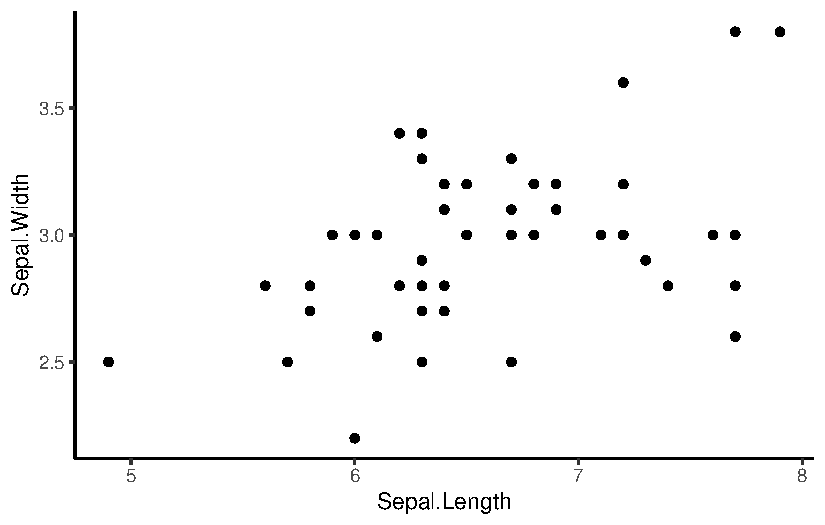
\includegraphics{cor_reg_chi_files/figure-pdf/unnamed-chunk-2-1.pdf}

}

\end{figure}

\hfill\break
\textbf{Step 2: Calculate a correlation coeficient (r)}

\begin{Shaded}
\begin{Highlighting}[]
\FunctionTok{cor}\NormalTok{(virg}\SpecialCharTok{$}\NormalTok{Sepal.Length, virg}\SpecialCharTok{$}\NormalTok{Sepal.Width)}
\end{Highlighting}
\end{Shaded}

\begin{verbatim}
[1] 0.4572278
\end{verbatim}

This value (r=0.45) positive and middle of the road/strong. This tells
us that some correlation likely exists.

\textbf{Step 3: Do a hypothesis test on the correlation}
\textbf{Spearman's Test}\\
H0: The correlation between these two variables is 0\\
Ha: The correlation != 0\\

\begin{Shaded}
\begin{Highlighting}[]
\FunctionTok{cor.test}\NormalTok{(virg}\SpecialCharTok{$}\NormalTok{Sepal.Length, virg}\SpecialCharTok{$}\NormalTok{Sepal.Width, }\AttributeTok{method=}\StringTok{"spearman"}\NormalTok{)}
\end{Highlighting}
\end{Shaded}

\begin{verbatim}
Warning in cor.test.default(virg$Sepal.Length, virg$Sepal.Width, method =
"spearman"): Cannot compute exact p-value with ties
\end{verbatim}

\begin{verbatim}

    Spearman's rank correlation rho

data:  virg$Sepal.Length and virg$Sepal.Width
S = 11943, p-value = 0.002011
alternative hypothesis: true rho is not equal to 0
sample estimates:
      rho 
0.4265165 
\end{verbatim}

The above output gives us the r value (cor=0.457) AND a p-value for a
hypothesis test that the two correlations do not differ. If
p\textless0.05 we can reject our H0 and say that the correlation differs
from 0. Here, p=0.0008 so we can reject H0 and suggest that we have a
significant positive correlation! Rho is similar to r and is this case
our correlation coefficient (0.42). It is slightly lower than the r we
calculated above.

\subsection{Multiple Correlations}

\begin{Shaded}
\begin{Highlighting}[]
\NormalTok{iris2}\OtherTok{\textless{}{-}}\NormalTok{iris[,}\FunctionTok{c}\NormalTok{(}\DecValTok{1}\SpecialCharTok{:}\DecValTok{4}\NormalTok{)] }\CommentTok{\#filter iris so we only have the numerical columns!}

\NormalTok{iris\_cor}\OtherTok{\textless{}{-}}\FunctionTok{cor}\NormalTok{(iris2, }\AttributeTok{method=}\StringTok{"spearman"}\NormalTok{)}

\NormalTok{iris\_cor}
\end{Highlighting}
\end{Shaded}

\begin{verbatim}
             Sepal.Length Sepal.Width Petal.Length Petal.Width
Sepal.Length    1.0000000  -0.1667777    0.8818981   0.8342888
Sepal.Width    -0.1667777   1.0000000   -0.3096351  -0.2890317
Petal.Length    0.8818981  -0.3096351    1.0000000   0.9376668
Petal.Width     0.8342888  -0.2890317    0.9376668   1.0000000
\end{verbatim}

The above correlation matrix shows r (correlation coefficient) not p
values!

\textbf{Getting r and p values}

\begin{Shaded}
\begin{Highlighting}[]
\NormalTok{mydata.rcorr }\OtherTok{=} \FunctionTok{rcorr}\NormalTok{(}\FunctionTok{as.matrix}\NormalTok{(iris2))}
\NormalTok{mydata.rcorr }\CommentTok{\#top matrix = r, bottom matrix = p}
\end{Highlighting}
\end{Shaded}

\begin{verbatim}
             Sepal.Length Sepal.Width Petal.Length Petal.Width
Sepal.Length         1.00       -0.12         0.87        0.82
Sepal.Width         -0.12        1.00        -0.43       -0.37
Petal.Length         0.87       -0.43         1.00        0.96
Petal.Width          0.82       -0.37         0.96        1.00

n= 150 


P
             Sepal.Length Sepal.Width Petal.Length Petal.Width
Sepal.Length              0.1519      0.0000       0.0000     
Sepal.Width  0.1519                   0.0000       0.0000     
Petal.Length 0.0000       0.0000                   0.0000     
Petal.Width  0.0000       0.0000      0.0000                  
\end{verbatim}

\textbf{Plotting our correlations}

\begin{Shaded}
\begin{Highlighting}[]
\FunctionTok{corrplot}\NormalTok{(iris\_cor)}
\end{Highlighting}
\end{Shaded}

\begin{figure}[H]

{\centering 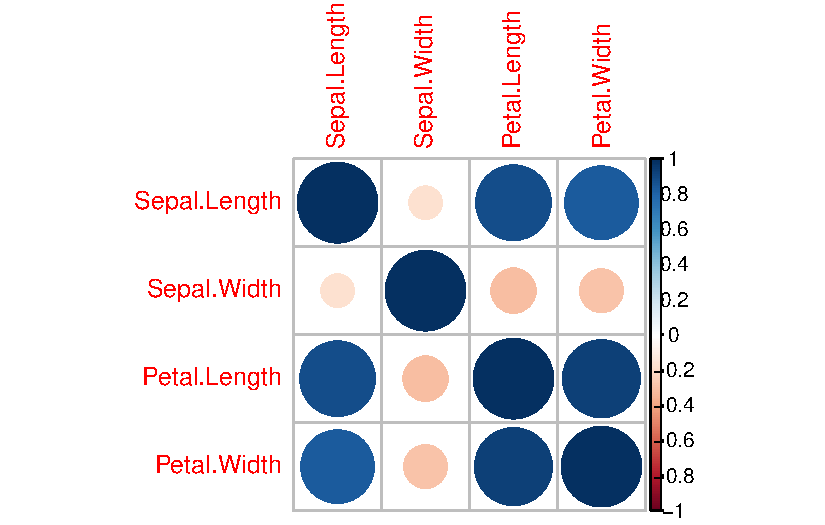
\includegraphics{cor_reg_chi_files/figure-pdf/unnamed-chunk-7-1.pdf}

}

\end{figure}

\subsection{Categorical correlations (Chi-Square)}

A Chi-square test is a statistical test used to determine if two
categorical variables have a significant correlation between them. These
two variables should be selected from the same population. An example -
Is the color of a thing red or green? Is the answer to a simple question
yes or no?\\
\strut \\
\textbf{Data format} Technically, a chi-square test is done on data that
are in a contingency table (contains columns (variables) in which
numbers represent counts. For example, here is a contingency table of
household chore data (exciting)

\begin{Shaded}
\begin{Highlighting}[]
\NormalTok{chore }\OtherTok{\textless{}{-}} \FunctionTok{read.delim}\NormalTok{(}\StringTok{"http://www.sthda.com/sthda/RDoc/data/housetasks.txt"}\NormalTok{, }\AttributeTok{row.names=}\DecValTok{1}\NormalTok{)}
\NormalTok{chore}
\end{Highlighting}
\end{Shaded}

\begin{verbatim}
           Wife Alternating Husband Jointly
Laundry     156          14       2       4
Main_meal   124          20       5       4
Dinner       77          11       7      13
Breakfeast   82          36      15       7
Tidying      53          11       1      57
Dishes       32          24       4      53
Shopping     33          23       9      55
Official     12          46      23      15
Driving      10          51      75       3
Finances     13          13      21      66
Insurance     8           1      53      77
Repairs       0           3     160       2
Holidays      0           1       6     153
\end{verbatim}

\textbf{H0} = The row and column data of the contingency table are
independent (no relationship) \textbf{Ha}= Row and column variables are
dependent (there is a relationship between them)

\textbf{The test}

\begin{Shaded}
\begin{Highlighting}[]
\NormalTok{chorechi}\OtherTok{\textless{}{-}}\FunctionTok{chisq.test}\NormalTok{(chore)}
\NormalTok{chorechi}
\end{Highlighting}
\end{Shaded}

\begin{verbatim}

    Pearson's Chi-squared test

data:  chore
X-squared = 1944.5, df = 36, p-value < 2.2e-16
\end{verbatim}

This result demonstrates that there is a significant association between
the columns and rows in the data (they are dependent).\\

\textbf{A second example}

Let's try to assess correlation between two categorical variables in a
dataframe we know! We will use mtcars

\begin{Shaded}
\begin{Highlighting}[]
\FunctionTok{head}\NormalTok{(mtcars)}
\end{Highlighting}
\end{Shaded}

\begin{verbatim}
                   mpg cyl disp  hp drat    wt  qsec vs am gear carb
Mazda RX4         21.0   6  160 110 3.90 2.620 16.46  0  1    4    4
Mazda RX4 Wag     21.0   6  160 110 3.90 2.875 17.02  0  1    4    4
Datsun 710        22.8   4  108  93 3.85 2.320 18.61  1  1    4    1
Hornet 4 Drive    21.4   6  258 110 3.08 3.215 19.44  1  0    3    1
Hornet Sportabout 18.7   8  360 175 3.15 3.440 17.02  0  0    3    2
Valiant           18.1   6  225 105 2.76 3.460 20.22  1  0    3    1
\end{verbatim}

\begin{Shaded}
\begin{Highlighting}[]
\CommentTok{\#make a contingency table}
\NormalTok{cartab}\OtherTok{\textless{}{-}}\FunctionTok{table}\NormalTok{(mtcars}\SpecialCharTok{$}\NormalTok{carb, mtcars}\SpecialCharTok{$}\NormalTok{cyl)}

\FunctionTok{chisq.test}\NormalTok{(cartab)}
\end{Highlighting}
\end{Shaded}

\begin{verbatim}
Warning in chisq.test(cartab): Chi-squared approximation may be incorrect
\end{verbatim}

\begin{verbatim}

    Pearson's Chi-squared test

data:  cartab
X-squared = 24.389, df = 10, p-value = 0.006632
\end{verbatim}

\begin{Shaded}
\begin{Highlighting}[]
\CommentTok{\#note that we don\textquotesingle{}t NEED to make the table. We can just do this}
\FunctionTok{chisq.test}\NormalTok{(mtcars}\SpecialCharTok{$}\NormalTok{carb, mtcars}\SpecialCharTok{$}\NormalTok{cyl)}
\end{Highlighting}
\end{Shaded}

\begin{verbatim}
Warning in chisq.test(mtcars$carb, mtcars$cyl): Chi-squared approximation may
be incorrect
\end{verbatim}

\begin{verbatim}

    Pearson's Chi-squared test

data:  mtcars$carb and mtcars$cyl
X-squared = 24.389, df = 10, p-value = 0.006632
\end{verbatim}

Both tests above are the same (just two options for you). We see that
p\textless0.05, thus we have evidence to reject H0 and suggest that carb
and cyl are dependent / correlated.

\hypertarget{simple-linear-regression}{%
\section{\texorpdfstring{\textbf{3. (Simple) Linear
Regression}}{3. (Simple) Linear Regression}}\label{simple-linear-regression}}

\subsection{plotting a regression line}

It is very easy to make a regression line in ggplot. We can plot our
scatterplot as we normally would and then we add the regression line
using the geom\_smooth() argument.

\begin{Shaded}
\begin{Highlighting}[]
\FunctionTok{ggplot}\NormalTok{(iris, }\FunctionTok{aes}\NormalTok{(}\AttributeTok{x=}\NormalTok{Petal.Length, }\AttributeTok{y=}\NormalTok{Sepal.Length))}\SpecialCharTok{+}
  \FunctionTok{geom\_point}\NormalTok{()}\SpecialCharTok{+}
  \FunctionTok{geom\_smooth}\NormalTok{(}\AttributeTok{method=}\StringTok{\textquotesingle{}lm\textquotesingle{}}\NormalTok{)}\SpecialCharTok{+}
  \FunctionTok{theme\_classic}\NormalTok{()}
\end{Highlighting}
\end{Shaded}

\begin{verbatim}
`geom_smooth()` using formula = 'y ~ x'
\end{verbatim}

\begin{figure}[H]

{\centering 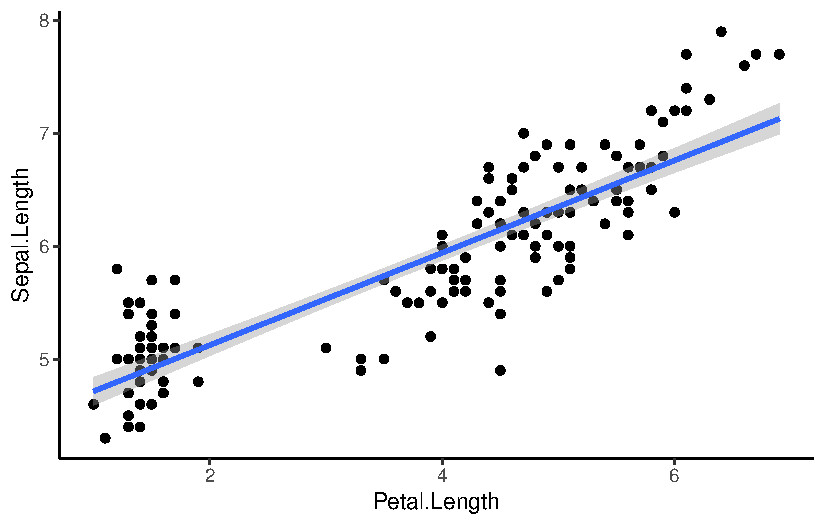
\includegraphics{cor_reg_chi_files/figure-pdf/unnamed-chunk-12-1.pdf}

}

\end{figure}

\hfill\break
The blue line represents our regression line (y\textasciitilde x). The
gray around the line is the SE. We can add SE=FALSE to our
geom\_smooth() to turn that off:

geom\_smooth(method=`lm', SE=FALSE)

\subsection{\texorpdfstring{\textbf{Assumptions}}{Assumptions}}

Linear regressions have 4 assumptions:

\textbf{1.)} Linearity of the data: We assume the relationship between
predictor (x) and outcome/dependent variable (y) is approx. linear. At
each value of X there is a population of possible Y-values whose mean
lies on the regression line.\\

\textbf{2.)} Normality of residuals: The residual error are assumed to
be normally distributed. In other words: at each value of X, the
distribution of possible Y values is normal\\

\textbf{3.)} Homogeneity of residual variance (homoscedasticity): We
assume residual variance is approx. constant. In other words: the
variance of Y values is the same at all values of X\\
\textbf{4.)} Independence of residual error terms: At each value of X,
the Y-measurements represent a random sample from the population of
possible Y values.\\

We can also make a residual plot to check some of our assumptions.
\textbf{Residuals} measure the scatter of points above or below the
least-squares regression line. When we calculate the residuals for a
linear regression and plot them, y=0 is the least squares line.
Residuals essentially represent the distance between each point and the
linear regression line we see in our regression graph.

\begin{Shaded}
\begin{Highlighting}[]
\FunctionTok{residuals}\NormalTok{(lm1)}
\end{Highlighting}
\end{Shaded}

\begin{verbatim}
          1           2           3           4           5           6 
 0.22090540  0.02090540 -0.13820238 -0.31998683  0.12090540  0.39822871 
          7           8           9          10          11          12 
-0.27909460  0.08001317 -0.47909460 -0.01998683  0.48001317 -0.16087906 
         13          14          15          16          17          18 
-0.07909460 -0.45641792  1.00268985  0.78001317  0.56179762  0.22090540 
         19          20          21          22          23          24 
 0.69822871  0.18001317  0.39822871  0.18001317 -0.11552569  0.09822871 
         25          26          27          28          29          30 
-0.28355574  0.03912094  0.03912094  0.28001317  0.32090540 -0.26087906 
         31          32          33          34          35          36 
-0.16087906  0.48001317  0.28001317  0.62090540 -0.01998683  0.20268985 
         37          38          39          40          41          42 
 0.66179762  0.02090540 -0.43820238  0.18001317  0.16179762 -0.33820238 
         43          44          45          46          47          48 
-0.43820238  0.03912094  0.01644426 -0.07909460  0.13912094 -0.27909460 
         49          50          51          52          53          54 
 0.38001317  0.12090540  0.77146188  0.25324634  0.58967743 -0.44229252 
         55          56          57          58          59          60 
 0.31235411 -0.44675366  0.07146188 -0.75604693  0.41235411 -0.70140030 
         61          62          63          64          65          66 
-0.73783139 -0.12407698  0.05770748 -0.12853812 -0.17872361  0.59413856 
         67          68          69          70          71          72 
-0.54675366 -0.18318475  0.05324634 -0.30140030 -0.36943035  0.15770748 
         73          74          75          76          77          78 
-0.01032257 -0.12853812  0.33503079  0.49413856  0.53056965  0.34878520 
         79          80          81          82          83          84 
-0.14675366 -0.03783139 -0.36050807 -0.31961584 -0.10140030 -0.39210703 
         85          86          87          88          89          90 
-0.74675366 -0.14675366  0.47146188  0.19413856 -0.38318475 -0.44229252 
         91          92          93          94          95          96 
-0.60586144 -0.08764589 -0.14229252 -0.65604693 -0.42407698 -0.32407698 
         97          98          99         100         101         102 
-0.32407698  0.13503079 -0.43337025 -0.28318475 -0.46013708 -0.59210703 
        103         104         105         106         107         108 
 0.38075515 -0.29656817 -0.17835262  0.59450955 -1.24675366  0.41718624 
        109         110         111         112         113         114 
 0.02164738  0.39897069  0.10789297 -0.07389149  0.24432406 -0.65121480 
        115         116         117         118         119         120 
-0.59210703 -0.07389149 -0.05567594  0.65361733  0.57183287 -0.35121480 
        121         122         123         124         125         126 
 0.26253960 -0.71032257  0.65361733 -0.01032257  0.06253960  0.43986292 
        127         128         129         130         131         132 
-0.06943035 -0.21032257 -0.19656817  0.52164738  0.59897069  0.97629401 
        133         134         135         136         137         138 
-0.19656817 -0.09210703 -0.49656817  0.89897069 -0.29656817 -0.15567594 
        139         140         141         142         143         144 
-0.26943035  0.38521629  0.10343183  0.50789297 -0.59210703  0.08075515 
        145         146         147         148         149         150 
 0.06253960  0.26700074 -0.05121480  0.06700074 -0.31478371 -0.49210703 
\end{verbatim}

\begin{Shaded}
\begin{Highlighting}[]
\FunctionTok{ggplot}\NormalTok{(lm1, }\FunctionTok{aes}\NormalTok{(}\AttributeTok{x=}\NormalTok{.fitted, }\AttributeTok{y=}\NormalTok{.resid))}\SpecialCharTok{+}
  \FunctionTok{geom\_point}\NormalTok{()}\SpecialCharTok{+}
  \FunctionTok{geom\_hline}\NormalTok{(}\AttributeTok{yintercept=}\DecValTok{0}\NormalTok{, }\AttributeTok{linetype=}\StringTok{\textquotesingle{}dashed\textquotesingle{}}\NormalTok{)}\SpecialCharTok{+}
  \FunctionTok{labs}\NormalTok{(}\AttributeTok{x=}\StringTok{\textquotesingle{}Petal Legnth\textquotesingle{}}\NormalTok{, }\AttributeTok{y=}\StringTok{\textquotesingle{}Residuals\textquotesingle{}}\NormalTok{)}\SpecialCharTok{+}
  \FunctionTok{theme\_classic}\NormalTok{()}
\end{Highlighting}
\end{Shaded}

\begin{figure}[H]

{\centering 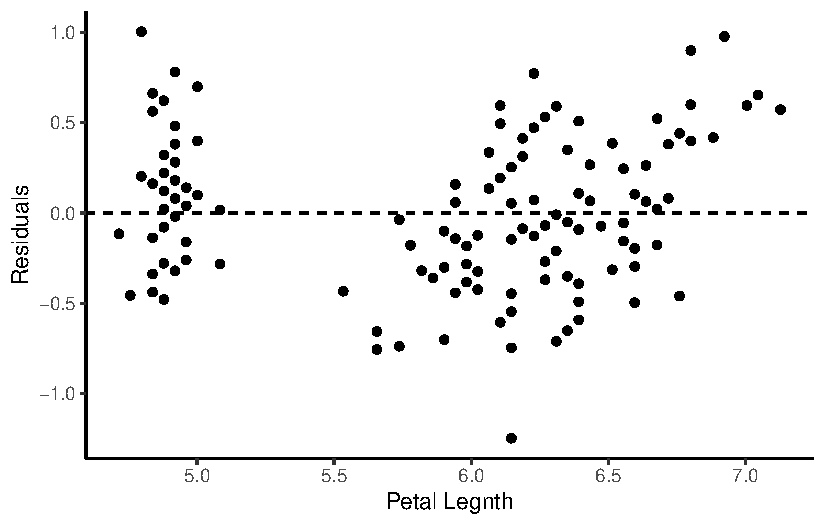
\includegraphics{cor_reg_chi_files/figure-pdf/unnamed-chunk-13-1.pdf}

}

\end{figure}

\hfill\break
If assumptions of normality and equal variance are met, a residual plot
should have: - A roughly symmetric cloud of points above and below the
horizontal line at 0 with a higher density of points close to the line
ran away from it.\\
- Little noticeable curvature as we move from left to right\\
- Approx. equal variance of points above and below the line at all
values of X\\
\strut \\

The residual plot above shows meets all assumptions, though this
analysis is somewhat subjective.

\textbf{An alternative assumption check} I think it is easier to do a
more comprehensive visual check with the performance package in R. We
can easily visually check the first 3 assumptions using check\_model().
Assumption 4 requires us to think about experimental design.

\begin{Shaded}
\begin{Highlighting}[]
\NormalTok{lm1}\OtherTok{\textless{}{-}}\FunctionTok{lm}\NormalTok{(Sepal.Length }\SpecialCharTok{\textasciitilde{}}\NormalTok{ Petal.Length, }\AttributeTok{data=}\NormalTok{iris)}

\FunctionTok{check\_model}\NormalTok{(lm1)}
\end{Highlighting}
\end{Shaded}

\begin{verbatim}
Not enough model terms in the conditional part of the model to check for
  multicollinearity.
\end{verbatim}

\begin{figure}[H]

{\centering 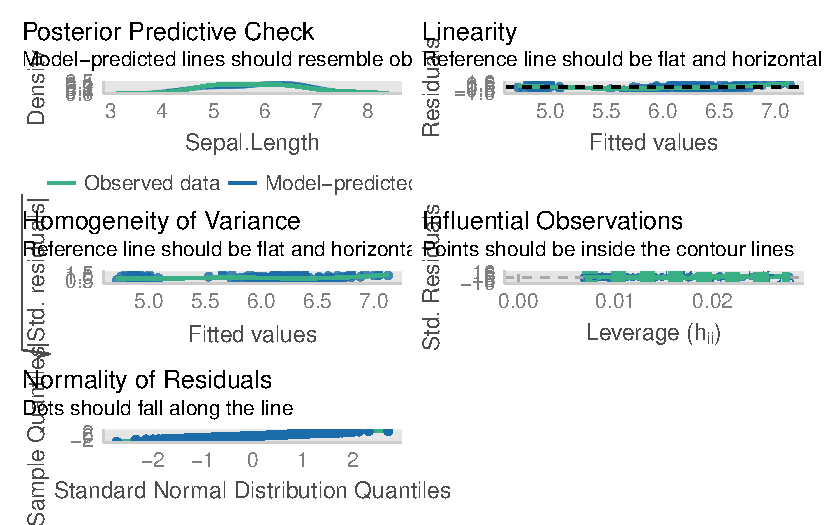
\includegraphics{cor_reg_chi_files/figure-pdf/unnamed-chunk-14-1.pdf}

}

\end{figure}

\hfill\break
Using the plots above, we can check 3 / 4 of our assumptions and look
for influential observations/outliers. The plots even tell us what to
look for on them! This is a bit simpler than trying to analyze the
residual plot.\\
As with the residual plot, this analysis of assumptions is somewhat
subjective. That is ok.

\subsection{\texorpdfstring{\textbf{when data are not
linear}}{when data are not linear}}

Sometimes the relationship between two variables is not linear! There
are many types of common relationships including logarithmic and
exponential. We can often visualize these relationships and
\textbf{Transform} our data to make them linear with some simple math.

Let's look at an example:

\begin{Shaded}
\begin{Highlighting}[]
\FunctionTok{head}\NormalTok{(Loblolly)}
\end{Highlighting}
\end{Shaded}

\begin{verbatim}
Grouped Data: height ~ age | Seed
   height age Seed
1    4.51   3  301
15  10.89   5  301
29  28.72  10  301
43  41.74  15  301
57  52.70  20  301
71  60.92  25  301
\end{verbatim}

\begin{Shaded}
\begin{Highlighting}[]
\NormalTok{p1}\OtherTok{\textless{}{-}}\FunctionTok{ggplot}\NormalTok{(Loblolly, }\FunctionTok{aes}\NormalTok{(}\AttributeTok{x=}\NormalTok{age, }\AttributeTok{y=}\NormalTok{height))}\SpecialCharTok{+}
  \FunctionTok{geom\_point}\NormalTok{()}\SpecialCharTok{+}
  \FunctionTok{geom\_smooth}\NormalTok{()}\SpecialCharTok{+}
  \FunctionTok{geom\_smooth}\NormalTok{(}\AttributeTok{method=}\StringTok{\textquotesingle{}lm\textquotesingle{}}\NormalTok{, }\AttributeTok{linetype=}\StringTok{\textquotesingle{}dashed\textquotesingle{}}\NormalTok{, }\AttributeTok{color=}\StringTok{\textquotesingle{}firebrick\textquotesingle{}}\NormalTok{)}\SpecialCharTok{+}
  \FunctionTok{theme\_classic}\NormalTok{()}\SpecialCharTok{+}
  \FunctionTok{labs}\NormalTok{(}\AttributeTok{title=}\StringTok{\textquotesingle{}original\textquotesingle{}}\NormalTok{)}
\CommentTok{\#this is roughly logarithmic in shape}

\NormalTok{lob}\OtherTok{\textless{}{-}}\NormalTok{Loblolly}
\NormalTok{lob}\SpecialCharTok{$}\NormalTok{age2}\OtherTok{\textless{}{-}}\FunctionTok{log}\NormalTok{(lob}\SpecialCharTok{$}\NormalTok{age)}

\NormalTok{p2}\OtherTok{\textless{}{-}}\FunctionTok{ggplot}\NormalTok{(lob, }\FunctionTok{aes}\NormalTok{(}\AttributeTok{x=}\NormalTok{age2, }\AttributeTok{y=}\NormalTok{height))}\SpecialCharTok{+}
  \FunctionTok{geom\_point}\NormalTok{()}\SpecialCharTok{+}
  \FunctionTok{geom\_smooth}\NormalTok{()}\SpecialCharTok{+}
  \FunctionTok{geom\_smooth}\NormalTok{(}\AttributeTok{method=}\StringTok{\textquotesingle{}lm\textquotesingle{}}\NormalTok{, }\AttributeTok{linetype=}\StringTok{\textquotesingle{}dashed\textquotesingle{}}\NormalTok{, }\AttributeTok{color=}\StringTok{\textquotesingle{}firebrick\textquotesingle{}}\NormalTok{)}\SpecialCharTok{+}
  \FunctionTok{theme\_classic}\NormalTok{()}\SpecialCharTok{+}
  \FunctionTok{labs}\NormalTok{(}\AttributeTok{title=}\StringTok{\textquotesingle{}log transformed\textquotesingle{}}\NormalTok{)}

\NormalTok{lob}\SpecialCharTok{$}\NormalTok{age3}\OtherTok{=}\NormalTok{(lob}\SpecialCharTok{$}\NormalTok{age2)}\SpecialCharTok{\^{}}\DecValTok{2}
\NormalTok{p3}\OtherTok{\textless{}{-}}\FunctionTok{ggplot}\NormalTok{(lob, }\FunctionTok{aes}\NormalTok{(}\AttributeTok{x=}\NormalTok{age3, }\AttributeTok{y=}\NormalTok{height))}\SpecialCharTok{+}
  \FunctionTok{geom\_point}\NormalTok{()}\SpecialCharTok{+}
  \FunctionTok{geom\_smooth}\NormalTok{()}\SpecialCharTok{+}
  \FunctionTok{geom\_smooth}\NormalTok{(}\AttributeTok{method=}\StringTok{\textquotesingle{}lm\textquotesingle{}}\NormalTok{, }\AttributeTok{linetype=}\StringTok{\textquotesingle{}dashed\textquotesingle{}}\NormalTok{, }\AttributeTok{color=}\StringTok{\textquotesingle{}firebrick\textquotesingle{}}\NormalTok{)}\SpecialCharTok{+}
  \FunctionTok{theme\_classic}\NormalTok{()}\SpecialCharTok{+}
  \FunctionTok{labs}\NormalTok{(}\AttributeTok{title=}\StringTok{\textquotesingle{}squared\textquotesingle{}}\NormalTok{)}

\NormalTok{p1}\SpecialCharTok{/}\NormalTok{p2}\SpecialCharTok{/}\NormalTok{p3}
\end{Highlighting}
\end{Shaded}

\begin{verbatim}
`geom_smooth()` using method = 'loess' and formula = 'y ~ x'
`geom_smooth()` using formula = 'y ~ x'
`geom_smooth()` using method = 'loess' and formula = 'y ~ x'
`geom_smooth()` using formula = 'y ~ x'
`geom_smooth()` using method = 'loess' and formula = 'y ~ x'
`geom_smooth()` using formula = 'y ~ x'
\end{verbatim}

\begin{figure}[H]

{\centering 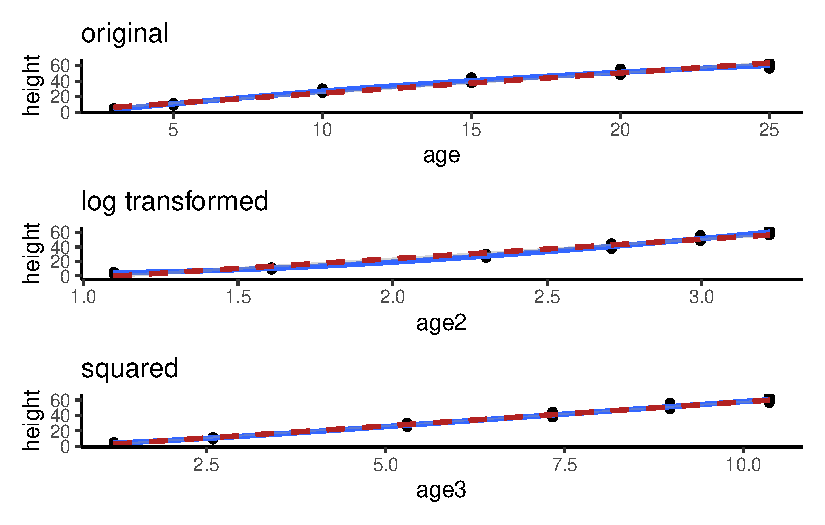
\includegraphics{cor_reg_chi_files/figure-pdf/unnamed-chunk-15-1.pdf}

}

\end{figure}

Here we can see that the transformation was fairly trivial (the data
were close enough to a straight line already). BUT, technically, the
first plot shows a logarithmic trend. We can transform one of the
variables to generate a more linear trend. We can guess a transformation
and check it with graphs or we can use our knowledge of mathematical
relationships to understand how we might make our relationship more
linear.

\subsection{\texorpdfstring{\textbf{Linear Regression with categorical
variables}}{Linear Regression with categorical variables}}

We can look at mtcars this time\ldots{}

\begin{Shaded}
\begin{Highlighting}[]
\FunctionTok{head}\NormalTok{(mtcars)}
\end{Highlighting}
\end{Shaded}

\begin{verbatim}
                   mpg cyl disp  hp drat    wt  qsec vs am gear carb
Mazda RX4         21.0   6  160 110 3.90 2.620 16.46  0  1    4    4
Mazda RX4 Wag     21.0   6  160 110 3.90 2.875 17.02  0  1    4    4
Datsun 710        22.8   4  108  93 3.85 2.320 18.61  1  1    4    1
Hornet 4 Drive    21.4   6  258 110 3.08 3.215 19.44  1  0    3    1
Hornet Sportabout 18.7   8  360 175 3.15 3.440 17.02  0  0    3    2
Valiant           18.1   6  225 105 2.76 3.460 20.22  1  0    3    1
\end{verbatim}

Now, I want to hypothesize that there will be no effect of cylinder on
horsepower (this is called a ``null hypothesis''). We've seen similar
hypothesis before in our ANOVA.

First, let's make cylinder a factor and plot a boxplot so we can see
whether there may be a trend here\ldots{}

\begin{Shaded}
\begin{Highlighting}[]
\NormalTok{mtcars}\SpecialCharTok{$}\NormalTok{cyl1}\OtherTok{=}\FunctionTok{as.factor}\NormalTok{(mtcars}\SpecialCharTok{$}\NormalTok{cyl)}

\FunctionTok{ggplot}\NormalTok{(mtcars, }\FunctionTok{aes}\NormalTok{(}\AttributeTok{x=}\NormalTok{cyl1, }\AttributeTok{y=}\NormalTok{hp))}\SpecialCharTok{+}
         \FunctionTok{geom\_boxplot}\NormalTok{()}\SpecialCharTok{+}
         \FunctionTok{theme\_bw}\NormalTok{()}
\end{Highlighting}
\end{Shaded}

\begin{figure}[H]

{\centering 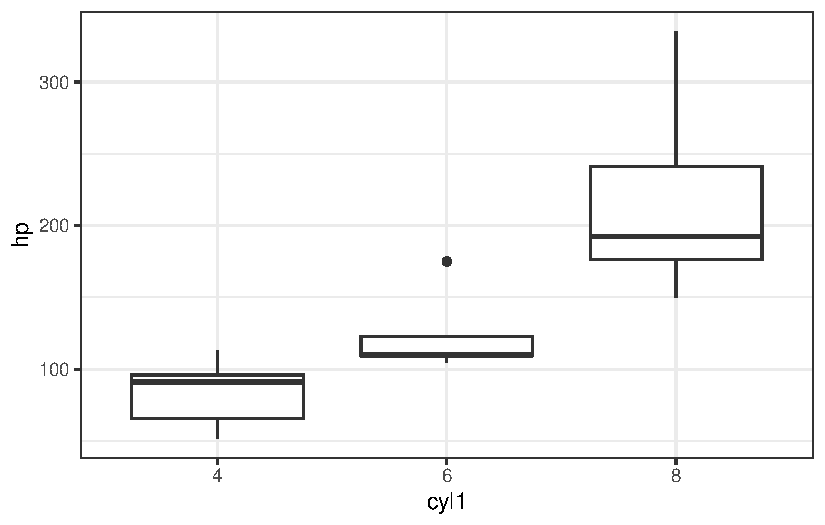
\includegraphics{cor_reg_chi_files/figure-pdf/unnamed-chunk-17-1.pdf}

}

\end{figure}

\hfill\break
I think it is safe to say we see what we might suspect to be a
linear(ish) relationship between cyl and hp, where hp increases as cyl
increases. What do you think?

Now, let's do some stats on this.

\subsection{\texorpdfstring{\textbf{Run the lm}}{Run the lm}}

\begin{Shaded}
\begin{Highlighting}[]
\NormalTok{lmhp}\OtherTok{\textless{}{-}}\FunctionTok{lm}\NormalTok{(hp}\SpecialCharTok{\textasciitilde{}}\NormalTok{cyl1, }\AttributeTok{data =}\NormalTok{ mtcars)}
\FunctionTok{summary}\NormalTok{(lmhp)}
\end{Highlighting}
\end{Shaded}

\begin{verbatim}

Call:
lm(formula = hp ~ cyl1, data = mtcars)

Residuals:
   Min     1Q Median     3Q    Max 
-59.21 -22.78  -8.25  15.97 125.79 

Coefficients:
            Estimate Std. Error t value Pr(>|t|)    
(Intercept)    82.64      11.43   7.228 5.86e-08 ***
cyl16          39.65      18.33   2.163   0.0389 *  
cyl18         126.58      15.28   8.285 3.92e-09 ***
---
Signif. codes:  0 '***' 0.001 '**' 0.01 '*' 0.05 '.' 0.1 ' ' 1

Residual standard error: 37.92 on 29 degrees of freedom
Multiple R-squared:  0.7139,    Adjusted R-squared:  0.6941 
F-statistic: 36.18 on 2 and 29 DF,  p-value: 1.319e-08
\end{verbatim}

This time we used a categorical x variable, which makes things a little
more interesting. In the coefficients table this time we see cyl = 6 and
cyl =8 represented as well as ``intercept.'' R takes the categorical
variables and places them in alpha numeric order in these tables. So
``intercept'' is actually cyl=4. The ``estimate'' tells us the effect
size of each category relative to ``intercept.'' SO, the mean of cyl=4
should be 82.64 (check the boxplot above to confirm). The mean of cyl=6
is not 39.65, but is actually 39.65 higher than mean of cyl=4 (82.64 +
39.65 = 132.29, which checks out). The p-values associated with each of
the coefficients test the null hypothesis that each coefficient has no
effect. A p \textless0.05 indicates that the coefficient is likely to be
meaningful in the model (changes in the predictor's value are related to
changes in the response value).

Further down, we see an R-squared of nearly 0.70, which is very good
evidence of a linear relationship (70\% of the variance in y can be
explained by x!). The p-value is very nearly 0.00, which indicates a
significant linear correlation.

\subsection{\texorpdfstring{\textbf{Check
assumptions!}}{Check assumptions!}}

\begin{Shaded}
\begin{Highlighting}[]
\FunctionTok{check\_model}\NormalTok{(lmhp)}
\end{Highlighting}
\end{Shaded}

\begin{verbatim}
Not enough model terms in the conditional part of the model to check for
  multicollinearity.
\end{verbatim}

\begin{figure}[H]

{\centering 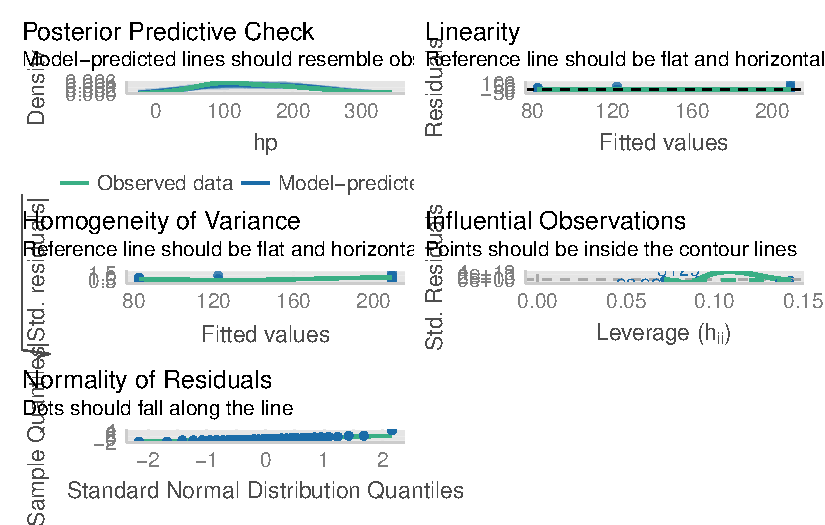
\includegraphics{cor_reg_chi_files/figure-pdf/unnamed-chunk-19-1.pdf}

}

\end{figure}

\hfill\break
Here we see some concern about Homoscedasticity and homogeneity of
variance. We can probably still assume our model is reliable, but we may
want to be careful. We learned ways to numerically assess this last
week, but again, with high enough sample size, this won't be an issue.
Here, I would suggest that n is too small, so if this were a real
statistical test we would have limitations to discuss.\\

Remember our hypothesis (null) was: ``There will be no effect of
cylinder on horsepower.'' We are able to reject this null hypothesis and
suggest that indeed horsepower increases as cylinder increases. We might
also add caveats that homoscedasticity was not confirmed due to low
sample size, but the result seems clear enough that this likely doesn't
matter.\\

\hypertarget{t-test}{%
\subsection{\texorpdfstring{\textbf{4.
t-test}}{4. t-test}}\label{t-test}}

\hypertarget{additional-tutorials-and-resources-for-t-tests}{%
\section{Additional Tutorials and Resources for
t-tests}\label{additional-tutorials-and-resources-for-t-tests}}

\href{https://statistics.berkeley.edu/computing/r-t-tests}{t-tests}

\subsection{\texorpdfstring{\textbf{A note on statistics and
experimental design}}{A note on statistics and experimental design}}

Statistics is a complex field with a long history. We could spend an
entire course or even an entire career focusing on the intricate details
of statistical decisions and ideas. We've already spent some time on
this! I want you to have the statistical grounding necessary to plan
your experiments and analyze your data. For biologists, statistics are a
tool we can leverage to perform the best possible experiments and test
our hypotheses. The T-test is the start of our stats journey. It's a
simple test and one that you may not use often, but the theory behind it
sets the stage for what is to come!

\hfill\break

\subsection{\texorpdfstring{\textbf{T-test theory}}{T-test theory}}

The t-test (or students' t-test) is a basic statistical test used to
assess whether or not the means of two groups are different from one
another. In this test, the null hypothesis is that the two means are
equal (or that there is no difference between the two means).

\textbf{A t-test should only be used if the following assumptions are
met:}\\
\textbf{1.)} the two distributions whose means we are comparing must be
\textbf{normally distributed}\\
\textbf{2.)} The variances of the two groups must be \textbf{equal}\\

\textbf{Generate example data}

\begin{Shaded}
\begin{Highlighting}[]
\NormalTok{iris2}\OtherTok{\textless{}{-}}\NormalTok{iris }\SpecialCharTok{\%\textgreater{}\%}
  \FunctionTok{filter}\NormalTok{(Species }\SpecialCharTok{!=} \StringTok{\textquotesingle{}setosa\textquotesingle{}}\NormalTok{) }\SpecialCharTok{\%\textgreater{}\%}
  \FunctionTok{droplevels}\NormalTok{() }\CommentTok{\#removes the empty levels so when we check levels below we only get the ones that are still in the data!}

\CommentTok{\#check levels to make sure we only have 2 species!}
\FunctionTok{head}\NormalTok{(iris2)}
\end{Highlighting}
\end{Shaded}

\begin{verbatim}
  Sepal.Length Sepal.Width Petal.Length Petal.Width    Species
1          7.0         3.2          4.7         1.4 versicolor
2          6.4         3.2          4.5         1.5 versicolor
3          6.9         3.1          4.9         1.5 versicolor
4          5.5         2.3          4.0         1.3 versicolor
5          6.5         2.8          4.6         1.5 versicolor
6          5.7         2.8          4.5         1.3 versicolor
\end{verbatim}

\begin{Shaded}
\begin{Highlighting}[]
\FunctionTok{levels}\NormalTok{(iris2}\SpecialCharTok{$}\NormalTok{Species)}
\end{Highlighting}
\end{Shaded}

\begin{verbatim}
[1] "versicolor" "virginica" 
\end{verbatim}

We will use these data for our examples today. T-test requires
\emph{only} 2 groups/populations. We will assess the alternative
hypothesis that one of our numerical variables (sepal length, sepal
width, petal length, or petal width) differs by species.

But first, we must \textbf{test our assumptions}

\subsection{\texorpdfstring{\textbf{Assumption 1.) Assessing
normality}}{Assumption 1.) Assessing normality}}

\emph{Method 1: the Shapiro-Wilk Test} If p \textless{} 0.05 then the
distribution is significantly different from normal.

Step 1: we need to create separate data frames for each species to
assess normality of each variable by species!

\begin{Shaded}
\begin{Highlighting}[]
\NormalTok{versi}\OtherTok{\textless{}{-}}\NormalTok{iris2 }\SpecialCharTok{\%\textgreater{}\%}
  \FunctionTok{filter}\NormalTok{(Species}\SpecialCharTok{==}\StringTok{\textquotesingle{}versicolor\textquotesingle{}}\NormalTok{) }\SpecialCharTok{\%\textgreater{}\%}
  \FunctionTok{droplevels}\NormalTok{()}

\NormalTok{virg}\OtherTok{\textless{}{-}}\NormalTok{iris2 }\SpecialCharTok{\%\textgreater{}\%}
  \FunctionTok{filter}\NormalTok{(Species}\SpecialCharTok{==}\StringTok{\textquotesingle{}virginica\textquotesingle{}}\NormalTok{) }\SpecialCharTok{\%\textgreater{}\%}
  \FunctionTok{droplevels}\NormalTok{()}
\end{Highlighting}
\end{Shaded}

\hfill\break

Step 2: We can run our shapiro-wilk tests on each variable if we'd like

\begin{Shaded}
\begin{Highlighting}[]
\FunctionTok{shapiro.test}\NormalTok{(versi}\SpecialCharTok{$}\NormalTok{Petal.Length) }\CommentTok{\#this is normally distributed}
\end{Highlighting}
\end{Shaded}

\begin{verbatim}

    Shapiro-Wilk normality test

data:  versi$Petal.Length
W = 0.966, p-value = 0.1585
\end{verbatim}

\begin{Shaded}
\begin{Highlighting}[]
\FunctionTok{shapiro.test}\NormalTok{(versi}\SpecialCharTok{$}\NormalTok{Petal.Width) }\CommentTok{\# this is not}
\end{Highlighting}
\end{Shaded}

\begin{verbatim}

    Shapiro-Wilk normality test

data:  versi$Petal.Width
W = 0.94763, p-value = 0.02728
\end{verbatim}

\begin{Shaded}
\begin{Highlighting}[]
\FunctionTok{shapiro.test}\NormalTok{(versi}\SpecialCharTok{$}\NormalTok{Sepal.Length) }\CommentTok{\#normal}
\end{Highlighting}
\end{Shaded}

\begin{verbatim}

    Shapiro-Wilk normality test

data:  versi$Sepal.Length
W = 0.97784, p-value = 0.4647
\end{verbatim}

\begin{Shaded}
\begin{Highlighting}[]
\FunctionTok{shapiro.test}\NormalTok{(versi}\SpecialCharTok{$}\NormalTok{Sepal.Width) }\CommentTok{\#normal}
\end{Highlighting}
\end{Shaded}

\begin{verbatim}

    Shapiro-Wilk normality test

data:  versi$Sepal.Width
W = 0.97413, p-value = 0.338
\end{verbatim}

\begin{Shaded}
\begin{Highlighting}[]
\FunctionTok{shapiro.test}\NormalTok{(virg}\SpecialCharTok{$}\NormalTok{Petal.Length) }\CommentTok{\#normal}
\end{Highlighting}
\end{Shaded}

\begin{verbatim}

    Shapiro-Wilk normality test

data:  virg$Petal.Length
W = 0.96219, p-value = 0.1098
\end{verbatim}

\begin{Shaded}
\begin{Highlighting}[]
\FunctionTok{shapiro.test}\NormalTok{(virg}\SpecialCharTok{$}\NormalTok{Petal.Width) }\CommentTok{\#normal}
\end{Highlighting}
\end{Shaded}

\begin{verbatim}

    Shapiro-Wilk normality test

data:  virg$Petal.Width
W = 0.95977, p-value = 0.08695
\end{verbatim}

\begin{Shaded}
\begin{Highlighting}[]
\FunctionTok{shapiro.test}\NormalTok{(virg}\SpecialCharTok{$}\NormalTok{Sepal.Length) }\CommentTok{\#normal}
\end{Highlighting}
\end{Shaded}

\begin{verbatim}

    Shapiro-Wilk normality test

data:  virg$Sepal.Length
W = 0.97118, p-value = 0.2583
\end{verbatim}

\begin{Shaded}
\begin{Highlighting}[]
\FunctionTok{shapiro.test}\NormalTok{(virg}\SpecialCharTok{$}\NormalTok{Sepal.Width) }\CommentTok{\#normal}
\end{Highlighting}
\end{Shaded}

\begin{verbatim}

    Shapiro-Wilk normality test

data:  virg$Sepal.Width
W = 0.96739, p-value = 0.1809
\end{verbatim}

\hfill\break
\emph{Method 2: Visualization}

Explore the following visualizations. Do you see clear evidence of
normality?

\begin{Shaded}
\begin{Highlighting}[]
\NormalTok{a1}\OtherTok{\textless{}{-}}\FunctionTok{ggplot}\NormalTok{(}\AttributeTok{data=}\NormalTok{iris2, }\FunctionTok{aes}\NormalTok{(Petal.Length, }\AttributeTok{fill=}\NormalTok{Species))}\SpecialCharTok{+}
  \FunctionTok{geom\_histogram}\NormalTok{(}\AttributeTok{binwidth =} \FloatTok{0.3}\NormalTok{)}\SpecialCharTok{+} 
  \FunctionTok{facet\_wrap}\NormalTok{(}\SpecialCharTok{\textasciitilde{}}\NormalTok{Species)}\SpecialCharTok{+}
  \FunctionTok{theme\_classic}\NormalTok{()}\SpecialCharTok{+}
  \FunctionTok{scale\_fill\_aaas}\NormalTok{()}

\NormalTok{a2}\OtherTok{\textless{}{-}}\FunctionTok{ggplot}\NormalTok{(}\AttributeTok{data=}\NormalTok{iris2, }\FunctionTok{aes}\NormalTok{(}\AttributeTok{x=}\NormalTok{Petal.Length, }\AttributeTok{y=}\NormalTok{Species, }\AttributeTok{fill=}\NormalTok{Species))}\SpecialCharTok{+}
  \FunctionTok{geom\_density\_ridges}\NormalTok{()}\SpecialCharTok{+} \CommentTok{\#makes a smooth density curve instead of a histogram!}
  \FunctionTok{theme\_classic}\NormalTok{()}\SpecialCharTok{+}
  \FunctionTok{scale\_fill\_aaas}\NormalTok{()}

\NormalTok{a1}\SpecialCharTok{/}\NormalTok{a2 }\CommentTok{\#compare the visualizations (they are of the same data){-} do we see normality here?}
\end{Highlighting}
\end{Shaded}

\begin{verbatim}
Picking joint bandwidth of 0.206
\end{verbatim}

\begin{figure}[H]

{\centering 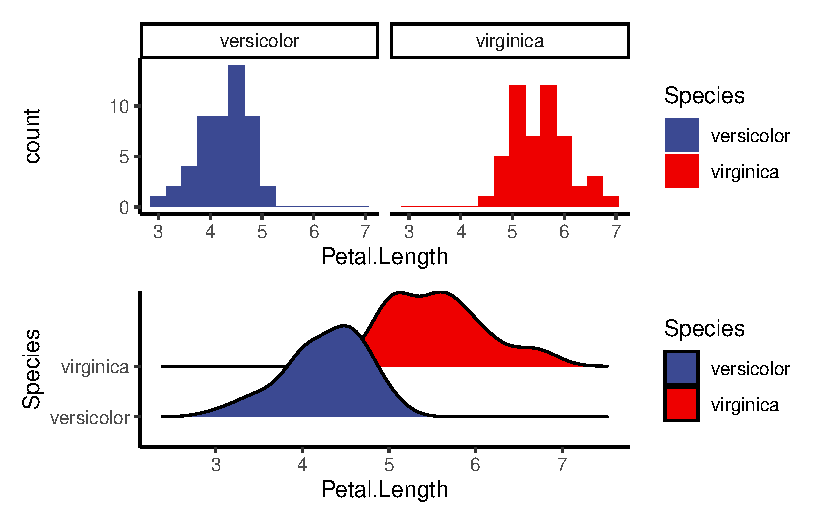
\includegraphics{cor_reg_chi_files/figure-pdf/unnamed-chunk-23-1.pdf}

}

\end{figure}

\begin{Shaded}
\begin{Highlighting}[]
\NormalTok{b1}\OtherTok{\textless{}{-}}\FunctionTok{ggplot}\NormalTok{(}\AttributeTok{data=}\NormalTok{iris2, }\FunctionTok{aes}\NormalTok{(Petal.Width, }\AttributeTok{fill=}\NormalTok{Species))}\SpecialCharTok{+}
  \FunctionTok{geom\_histogram}\NormalTok{(}\AttributeTok{binwidth =} \FloatTok{0.3}\NormalTok{)}\SpecialCharTok{+} 
  \FunctionTok{facet\_wrap}\NormalTok{(}\SpecialCharTok{\textasciitilde{}}\NormalTok{Species)}\SpecialCharTok{+}
  \FunctionTok{theme\_classic}\NormalTok{()}\SpecialCharTok{+}
  \FunctionTok{scale\_fill\_aaas}\NormalTok{()}

\NormalTok{b2}\OtherTok{\textless{}{-}}\FunctionTok{ggplot}\NormalTok{(}\AttributeTok{data=}\NormalTok{iris2, }\FunctionTok{aes}\NormalTok{(}\AttributeTok{x=}\NormalTok{Petal.Width, }\AttributeTok{y=}\NormalTok{Species, }\AttributeTok{fill=}\NormalTok{Species))}\SpecialCharTok{+}
  \FunctionTok{geom\_density\_ridges}\NormalTok{()}\SpecialCharTok{+} \CommentTok{\#makes a smooth density curve instead of a histogram!}
  \FunctionTok{theme\_classic}\NormalTok{()}\SpecialCharTok{+}
  \FunctionTok{scale\_fill\_aaas}\NormalTok{()}

\NormalTok{b1}\SpecialCharTok{/}\NormalTok{b2 }\CommentTok{\#compare the visualizations (they are of the same data){-} do we see normality here?}
\end{Highlighting}
\end{Shaded}

\begin{verbatim}
Picking joint bandwidth of 0.0972
\end{verbatim}

\begin{figure}[H]

{\centering 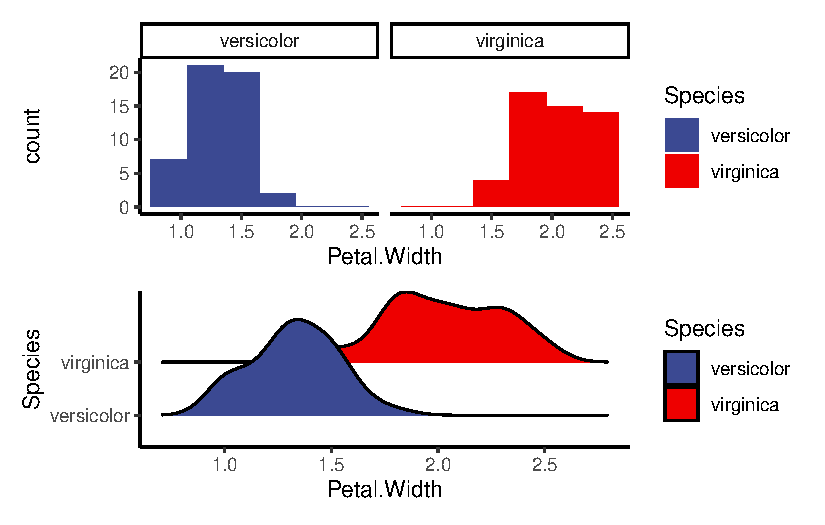
\includegraphics{cor_reg_chi_files/figure-pdf/unnamed-chunk-24-1.pdf}

}

\end{figure}

\begin{Shaded}
\begin{Highlighting}[]
\NormalTok{c1}\OtherTok{\textless{}{-}}\FunctionTok{ggplot}\NormalTok{(}\AttributeTok{data=}\NormalTok{iris2, }\FunctionTok{aes}\NormalTok{(Sepal.Width, }\AttributeTok{fill=}\NormalTok{Species))}\SpecialCharTok{+}
  \FunctionTok{geom\_histogram}\NormalTok{(}\AttributeTok{binwidth =} \FloatTok{0.3}\NormalTok{)}\SpecialCharTok{+} 
  \FunctionTok{facet\_wrap}\NormalTok{(}\SpecialCharTok{\textasciitilde{}}\NormalTok{Species)}\SpecialCharTok{+}
  \FunctionTok{theme\_classic}\NormalTok{()}\SpecialCharTok{+}
  \FunctionTok{scale\_fill\_aaas}\NormalTok{()}

\NormalTok{c2}\OtherTok{\textless{}{-}}\FunctionTok{ggplot}\NormalTok{(}\AttributeTok{data=}\NormalTok{iris2, }\FunctionTok{aes}\NormalTok{(}\AttributeTok{x=}\NormalTok{Sepal.Width, }\AttributeTok{y=}\NormalTok{Species, }\AttributeTok{fill=}\NormalTok{Species))}\SpecialCharTok{+}
  \FunctionTok{geom\_density\_ridges}\NormalTok{()}\SpecialCharTok{+} \CommentTok{\#makes a smooth density curve instead of a histogram!}
  \FunctionTok{theme\_classic}\NormalTok{()}\SpecialCharTok{+}
  \FunctionTok{scale\_fill\_aaas}\NormalTok{()}

\NormalTok{c1}\SpecialCharTok{/}\NormalTok{c2 }\CommentTok{\#compare the visualizations (they are of the same data){-} do we see normality here?}
\end{Highlighting}
\end{Shaded}

\begin{verbatim}
Picking joint bandwidth of 0.122
\end{verbatim}

\begin{figure}[H]

{\centering 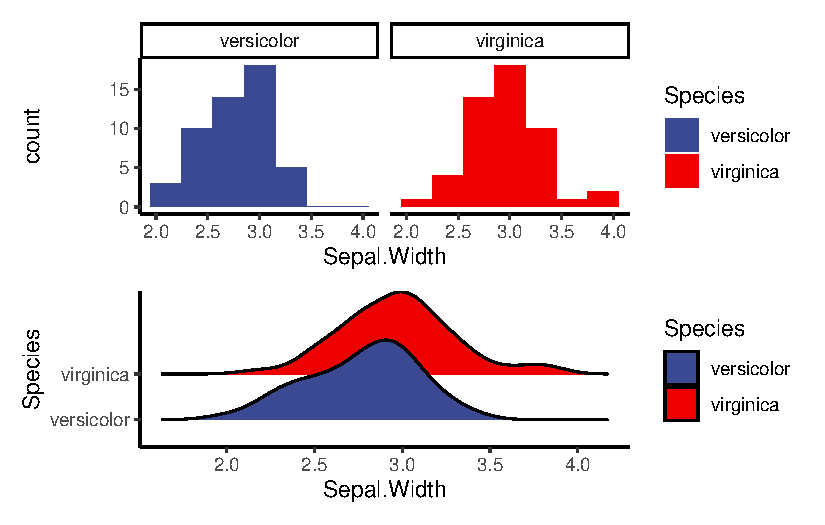
\includegraphics{cor_reg_chi_files/figure-pdf/unnamed-chunk-25-1.pdf}

}

\end{figure}

\begin{Shaded}
\begin{Highlighting}[]
\NormalTok{d1}\OtherTok{\textless{}{-}}\FunctionTok{ggplot}\NormalTok{(}\AttributeTok{data=}\NormalTok{iris2, }\FunctionTok{aes}\NormalTok{(Sepal.Length, }\AttributeTok{fill=}\NormalTok{Species))}\SpecialCharTok{+}
  \FunctionTok{geom\_histogram}\NormalTok{(}\AttributeTok{binwidth =} \FloatTok{0.3}\NormalTok{)}\SpecialCharTok{+} 
  \FunctionTok{facet\_wrap}\NormalTok{(}\SpecialCharTok{\textasciitilde{}}\NormalTok{Species)}\SpecialCharTok{+}
  \FunctionTok{theme\_classic}\NormalTok{()}\SpecialCharTok{+}
  \FunctionTok{scale\_fill\_aaas}\NormalTok{()}

\NormalTok{d2}\OtherTok{\textless{}{-}}\FunctionTok{ggplot}\NormalTok{(}\AttributeTok{data=}\NormalTok{iris2, }\FunctionTok{aes}\NormalTok{(}\AttributeTok{x=}\NormalTok{Sepal.Length, }\AttributeTok{y=}\NormalTok{Species, }\AttributeTok{fill=}\NormalTok{Species))}\SpecialCharTok{+}
  \FunctionTok{geom\_density\_ridges}\NormalTok{()}\SpecialCharTok{+} \CommentTok{\#makes a smooth density curve instead of a histogram!}
  \FunctionTok{theme\_classic}\NormalTok{()}\SpecialCharTok{+}
  \FunctionTok{scale\_fill\_aaas}\NormalTok{()}

\NormalTok{d1}\SpecialCharTok{/}\NormalTok{d2 }\CommentTok{\#compare the visualizations (they are of the same data){-} do we see normality here?}
\end{Highlighting}
\end{Shaded}

\begin{verbatim}
Picking joint bandwidth of 0.21
\end{verbatim}

\begin{figure}[H]

{\centering 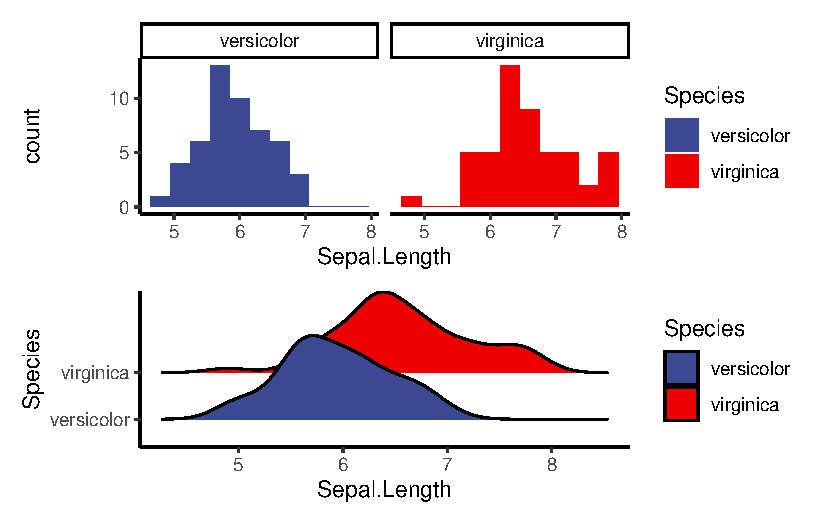
\includegraphics{cor_reg_chi_files/figure-pdf/unnamed-chunk-26-1.pdf}

}

\end{figure}

\subsection{\texorpdfstring{\textbf{Assumption 2.) Assessing equal
variance}}{Assumption 2.) Assessing equal variance}}

AKA homogeneity of variance\\

\textbf{Methods 1: F-test} We will use the \textbf{F-Test} to compare
the variance of two populations. This can only be used with \emph{2}
populations and is thus only useful when we run a t-test.

H0 for an F-test is: The variances of the two groups are equal.\\
Ha: The variances are different\\
p\textless0.05 allows us to reject the null (H0) and suggests that the
variances are different\\
\strut \\
\textbf{note:} The F-test assumes our data are already normal! You
should not run it on non-normal data

\begin{Shaded}
\begin{Highlighting}[]
\CommentTok{\#we use var.test to run an F{-}test}
\NormalTok{f1}\OtherTok{\textless{}{-}} \FunctionTok{var.test}\NormalTok{(Petal.Length }\SpecialCharTok{\textasciitilde{}}\NormalTok{ Species, }\AttributeTok{data=}\NormalTok{iris2)}
\NormalTok{f1 }\CommentTok{\# p\textgreater{}0.05, so we fail to reject H0 (the variances are likely equal)}
\end{Highlighting}
\end{Shaded}

\begin{verbatim}

    F test to compare two variances

data:  Petal.Length by Species
F = 0.72497, num df = 49, denom df = 49, p-value = 0.2637
alternative hypothesis: true ratio of variances is not equal to 1
95 percent confidence interval:
 0.411402 1.277530
sample estimates:
ratio of variances 
         0.7249678 
\end{verbatim}

\begin{Shaded}
\begin{Highlighting}[]
\NormalTok{f2}\OtherTok{\textless{}{-}} \FunctionTok{var.test}\NormalTok{(Petal.Width }\SpecialCharTok{\textasciitilde{}}\NormalTok{ Species, }\AttributeTok{data=}\NormalTok{iris2)}
\NormalTok{f2 }\CommentTok{\# p\textless{}0.05, so we reject H0 (variances are likely different)}
\end{Highlighting}
\end{Shaded}

\begin{verbatim}

    F test to compare two variances

data:  Petal.Width by Species
F = 0.51842, num df = 49, denom df = 49, p-value = 0.02335
alternative hypothesis: true ratio of variances is not equal to 1
95 percent confidence interval:
 0.2941935 0.9135614
sample estimates:
ratio of variances 
         0.5184243 
\end{verbatim}

\begin{Shaded}
\begin{Highlighting}[]
\NormalTok{f3}\OtherTok{\textless{}{-}} \FunctionTok{var.test}\NormalTok{(Sepal.Length }\SpecialCharTok{\textasciitilde{}}\NormalTok{ Species, }\AttributeTok{data=}\NormalTok{iris2)}
\NormalTok{f3 }\CommentTok{\# p\textgreater{}0.05, so we fail to reject H0 (the variances are likely equal)}
\end{Highlighting}
\end{Shaded}

\begin{verbatim}

    F test to compare two variances

data:  Sepal.Length by Species
F = 0.65893, num df = 49, denom df = 49, p-value = 0.1478
alternative hypothesis: true ratio of variances is not equal to 1
95 percent confidence interval:
 0.3739257 1.1611546
sample estimates:
ratio of variances 
         0.6589276 
\end{verbatim}

\begin{Shaded}
\begin{Highlighting}[]
\NormalTok{f4}\OtherTok{\textless{}{-}} \FunctionTok{var.test}\NormalTok{(Sepal.Width }\SpecialCharTok{\textasciitilde{}}\NormalTok{ Species, }\AttributeTok{data=}\NormalTok{iris2)}
\NormalTok{f4 }\CommentTok{\# p\textgreater{}0.05, so we fail to reject H0 (the variances are likely equal)}
\end{Highlighting}
\end{Shaded}

\begin{verbatim}

    F test to compare two variances

data:  Sepal.Width by Species
F = 0.94678, num df = 49, denom df = 49, p-value = 0.849
alternative hypothesis: true ratio of variances is not equal to 1
95 percent confidence interval:
 0.5372773 1.6684117
sample estimates:
ratio of variances 
         0.9467839 
\end{verbatim}

\hfill\break
\textbf{Method 2: Levene Test}\\
A more flexible test of homogeneity of variance is the Levene Test. It
can be used to compare the variance of many populations (not just 2) and
is more flexible than the F-test, so it can be used even if the
normality assumption is violated.\\
\textbf{this is the most commonly used test for homogeneity of
variance}\\
\textbf{leveneTest() is in the car package in R!}\\

N0: Variances of all populations are equal\\
p\textless0.05 allows us to reject H0

\begin{Shaded}
\begin{Highlighting}[]
\NormalTok{l1}\OtherTok{\textless{}{-}} \FunctionTok{leveneTest}\NormalTok{(Petal.Length }\SpecialCharTok{\textasciitilde{}}\NormalTok{ Species, }\AttributeTok{data=}\NormalTok{iris2)}
\NormalTok{l1 }\CommentTok{\# p\textgreater{}0.05, so we fail to reject H0 (the variances are likely equal)}
\end{Highlighting}
\end{Shaded}

\begin{verbatim}
Levene's Test for Homogeneity of Variance (center = median)
      Df F value Pr(>F)
group  1  1.0674 0.3041
      98               
\end{verbatim}

\begin{Shaded}
\begin{Highlighting}[]
\NormalTok{l2}\OtherTok{\textless{}{-}} \FunctionTok{leveneTest}\NormalTok{(Petal.Width }\SpecialCharTok{\textasciitilde{}}\NormalTok{ Species, }\AttributeTok{data=}\NormalTok{iris2)}
\NormalTok{l2 }\CommentTok{\# p\textless{}0.05, so we reject H0 (variances are likely different)}
\end{Highlighting}
\end{Shaded}

\begin{verbatim}
Levene's Test for Homogeneity of Variance (center = median)
      Df F value  Pr(>F)  
group  1  6.5455 0.01205 *
      98                  
---
Signif. codes:  0 '***' 0.001 '**' 0.01 '*' 0.05 '.' 0.1 ' ' 1
\end{verbatim}

\begin{Shaded}
\begin{Highlighting}[]
\NormalTok{l3}\OtherTok{\textless{}{-}} \FunctionTok{leveneTest}\NormalTok{(Sepal.Length }\SpecialCharTok{\textasciitilde{}}\NormalTok{ Species, }\AttributeTok{data=}\NormalTok{iris2)}
\NormalTok{l3 }\CommentTok{\# p\textgreater{}0.05, so we fail to reject H0 (the variances are likely equal)}
\end{Highlighting}
\end{Shaded}

\begin{verbatim}
Levene's Test for Homogeneity of Variance (center = median)
      Df F value Pr(>F)
group  1  1.0245 0.3139
      98               
\end{verbatim}

\begin{Shaded}
\begin{Highlighting}[]
\NormalTok{l4}\OtherTok{\textless{}{-}} \FunctionTok{leveneTest}\NormalTok{(Sepal.Width }\SpecialCharTok{\textasciitilde{}}\NormalTok{ Species, }\AttributeTok{data=}\NormalTok{iris2)}
\NormalTok{l4 }\CommentTok{\# p\textgreater{}0.05, so we fail to reject H0 (the variances are likely equal)}
\end{Highlighting}
\end{Shaded}

\begin{verbatim}
Levene's Test for Homogeneity of Variance (center = median)
      Df F value Pr(>F)
group  1  0.0873 0.7683
      98               
\end{verbatim}

\hfill\break
\textbf{Method 3: Visualization}\\
Since p-values are more like guidelines, we also want to visualize our
data to assess homogeneity of variance. We can do that in several ways.
You might already have some ideas about this! In general, it seems smart
to display the raw data as points and as boxplots. Let's start there!

\begin{Shaded}
\begin{Highlighting}[]
\NormalTok{v1}\FloatTok{.1}\OtherTok{\textless{}{-}}\FunctionTok{ggplot}\NormalTok{(}\AttributeTok{data=}\NormalTok{iris2, }\FunctionTok{aes}\NormalTok{(}\AttributeTok{x=}\NormalTok{Species, }\AttributeTok{y=}\NormalTok{Petal.Length, }\AttributeTok{color=}\NormalTok{Species))}\SpecialCharTok{+}
  \FunctionTok{geom\_point}\NormalTok{()}\SpecialCharTok{+}
  \FunctionTok{theme\_classic}\NormalTok{()}\SpecialCharTok{+}
  \FunctionTok{scale\_color\_aaas}\NormalTok{()}

\NormalTok{v1}\FloatTok{.2}\OtherTok{\textless{}{-}}\FunctionTok{ggplot}\NormalTok{(}\AttributeTok{data=}\NormalTok{iris2, }\FunctionTok{aes}\NormalTok{(}\AttributeTok{x=}\NormalTok{Species, }\AttributeTok{y=}\NormalTok{Petal.Length, }\AttributeTok{color=}\NormalTok{Species))}\SpecialCharTok{+}
  \FunctionTok{geom\_boxplot}\NormalTok{()}\SpecialCharTok{+}
  \FunctionTok{theme\_classic}\NormalTok{()}\SpecialCharTok{+}
  \FunctionTok{scale\_color\_aaas}\NormalTok{()}

\NormalTok{v1}\FloatTok{.1}\SpecialCharTok{+}\NormalTok{v1}\FloatTok{.2}
\end{Highlighting}
\end{Shaded}

\begin{figure}[H]

{\centering 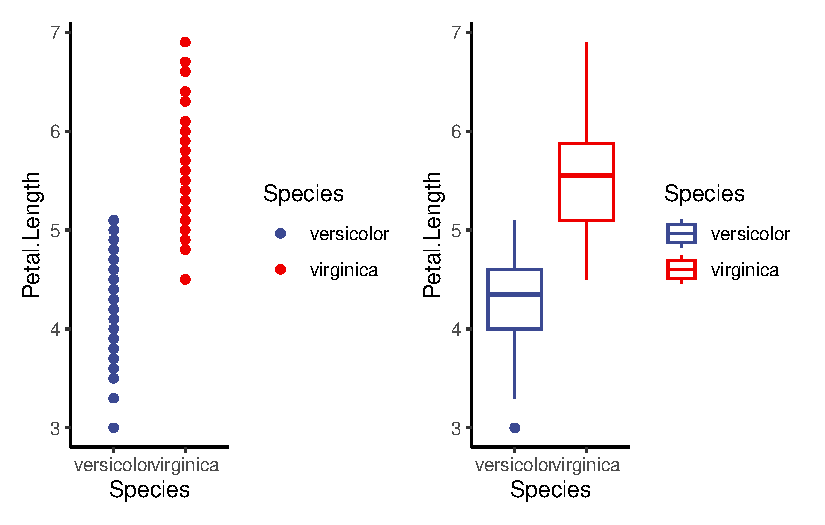
\includegraphics{cor_reg_chi_files/figure-pdf/unnamed-chunk-29-1.pdf}

}

\end{figure}

\begin{Shaded}
\begin{Highlighting}[]
\NormalTok{v2}\FloatTok{.1}\OtherTok{\textless{}{-}}\FunctionTok{ggplot}\NormalTok{(}\AttributeTok{data=}\NormalTok{iris2, }\FunctionTok{aes}\NormalTok{(}\AttributeTok{x=}\NormalTok{Species, }\AttributeTok{y=}\NormalTok{Petal.Width, }\AttributeTok{color=}\NormalTok{Species))}\SpecialCharTok{+}
  \FunctionTok{geom\_point}\NormalTok{()}\SpecialCharTok{+}
  \FunctionTok{theme\_classic}\NormalTok{()}\SpecialCharTok{+}
  \FunctionTok{scale\_color\_aaas}\NormalTok{()}

\NormalTok{v2}\FloatTok{.2}\OtherTok{\textless{}{-}}\FunctionTok{ggplot}\NormalTok{(}\AttributeTok{data=}\NormalTok{iris2, }\FunctionTok{aes}\NormalTok{(}\AttributeTok{x=}\NormalTok{Species, }\AttributeTok{y=}\NormalTok{Petal.Width, }\AttributeTok{color=}\NormalTok{Species))}\SpecialCharTok{+}
  \FunctionTok{geom\_boxplot}\NormalTok{()}\SpecialCharTok{+}
  \FunctionTok{theme\_classic}\NormalTok{()}\SpecialCharTok{+}
  \FunctionTok{scale\_color\_aaas}\NormalTok{()}

\NormalTok{v2}\FloatTok{.1}\SpecialCharTok{+}\NormalTok{v2}\FloatTok{.2}
\end{Highlighting}
\end{Shaded}

\begin{figure}[H]

{\centering 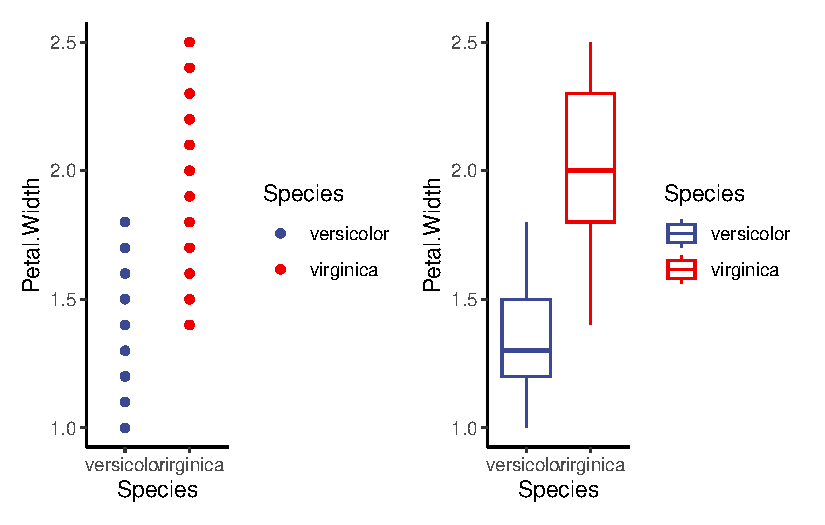
\includegraphics{cor_reg_chi_files/figure-pdf/unnamed-chunk-30-1.pdf}

}

\end{figure}

\begin{Shaded}
\begin{Highlighting}[]
\NormalTok{v3}\FloatTok{.1}\OtherTok{\textless{}{-}}\FunctionTok{ggplot}\NormalTok{(}\AttributeTok{data=}\NormalTok{iris2, }\FunctionTok{aes}\NormalTok{(}\AttributeTok{x=}\NormalTok{Species, }\AttributeTok{y=}\NormalTok{Sepal.Width, }\AttributeTok{color=}\NormalTok{Species))}\SpecialCharTok{+}
  \FunctionTok{geom\_point}\NormalTok{()}\SpecialCharTok{+}
  \FunctionTok{theme\_classic}\NormalTok{()}\SpecialCharTok{+}
  \FunctionTok{scale\_color\_aaas}\NormalTok{()}

\NormalTok{v3}\FloatTok{.2}\OtherTok{\textless{}{-}}\FunctionTok{ggplot}\NormalTok{(}\AttributeTok{data=}\NormalTok{iris2, }\FunctionTok{aes}\NormalTok{(}\AttributeTok{x=}\NormalTok{Species, }\AttributeTok{y=}\NormalTok{Sepal.Width, }\AttributeTok{color=}\NormalTok{Species))}\SpecialCharTok{+}
  \FunctionTok{geom\_boxplot}\NormalTok{()}\SpecialCharTok{+}
  \FunctionTok{theme\_classic}\NormalTok{()}\SpecialCharTok{+}
  \FunctionTok{scale\_color\_aaas}\NormalTok{()}

\NormalTok{v3}\FloatTok{.1}\SpecialCharTok{+}\NormalTok{v3}\FloatTok{.2}
\end{Highlighting}
\end{Shaded}

\begin{figure}[H]

{\centering 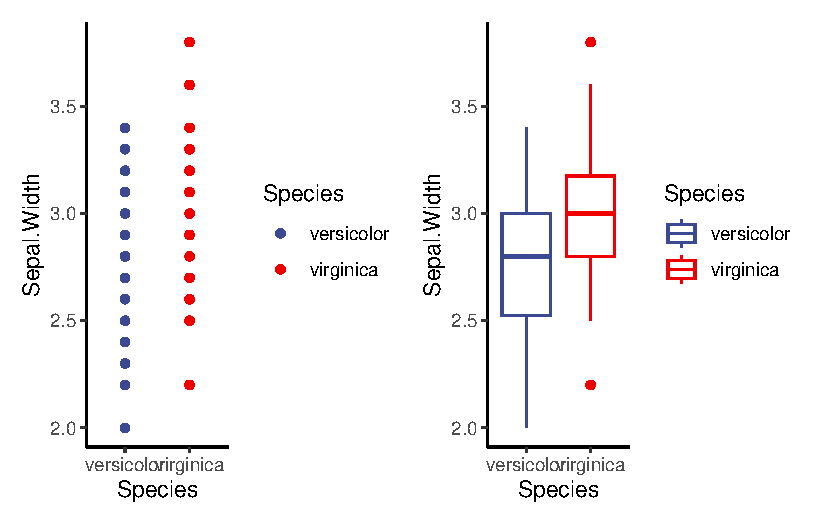
\includegraphics{cor_reg_chi_files/figure-pdf/unnamed-chunk-31-1.pdf}

}

\end{figure}

\begin{Shaded}
\begin{Highlighting}[]
\NormalTok{v4}\FloatTok{.1}\OtherTok{\textless{}{-}}\FunctionTok{ggplot}\NormalTok{(}\AttributeTok{data=}\NormalTok{iris2, }\FunctionTok{aes}\NormalTok{(}\AttributeTok{x=}\NormalTok{Species, }\AttributeTok{y=}\NormalTok{Sepal.Length, }\AttributeTok{color=}\NormalTok{Species))}\SpecialCharTok{+}
  \FunctionTok{geom\_point}\NormalTok{()}\SpecialCharTok{+}
  \FunctionTok{theme\_classic}\NormalTok{()}\SpecialCharTok{+}
  \FunctionTok{scale\_color\_aaas}\NormalTok{()}

\NormalTok{v4}\FloatTok{.2}\OtherTok{\textless{}{-}}\FunctionTok{ggplot}\NormalTok{(}\AttributeTok{data=}\NormalTok{iris2, }\FunctionTok{aes}\NormalTok{(}\AttributeTok{x=}\NormalTok{Species, }\AttributeTok{y=}\NormalTok{Sepal.Length, }\AttributeTok{color=}\NormalTok{Species))}\SpecialCharTok{+}
  \FunctionTok{geom\_boxplot}\NormalTok{()}\SpecialCharTok{+}
  \FunctionTok{theme\_classic}\NormalTok{()}\SpecialCharTok{+}
  \FunctionTok{scale\_color\_aaas}\NormalTok{()}

\NormalTok{v4}\FloatTok{.1}\SpecialCharTok{+}\NormalTok{v4}\FloatTok{.2}
\end{Highlighting}
\end{Shaded}

\begin{figure}[H]

{\centering 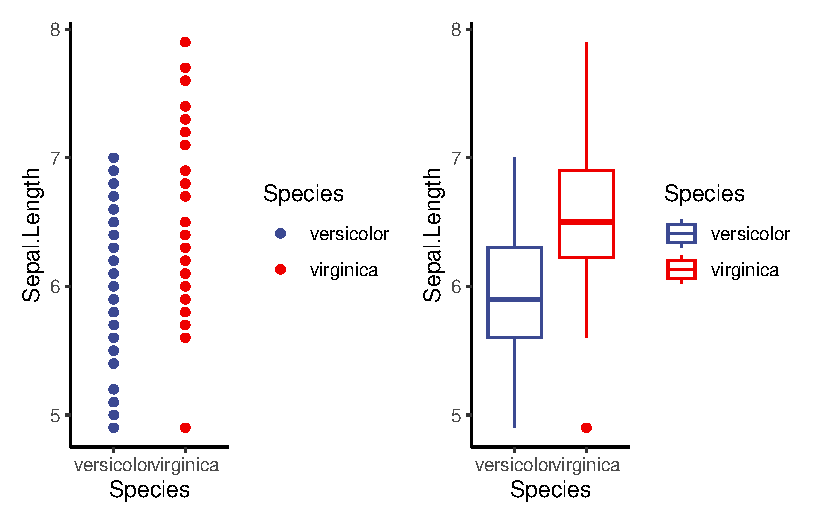
\includegraphics{cor_reg_chi_files/figure-pdf/unnamed-chunk-32-1.pdf}

}

\end{figure}

\subsection{\texorpdfstring{\textbf{When can we ignore
assumptions?}}{When can we ignore assumptions?}}

We can if our sample sizes are large. If n is small, we should not
ignore this assumption. There are alternatives to dealing with normality
that we can discuss in the ANOVA section (such as transforming the data)

\href{https://thestatsgeek.com/2013/09/28/the-t-test-and-robustness-to-non-normality/}{For
more info on that}

We can also ignore the equal variance requirement if we use the Welch
t-test (default in R)\\

\subsection{\texorpdfstring{\textbf{A basic T-test in
R}}{A basic T-test in R}}

Finally, let's do some T-tests!\\

H0: No difference between the means of the 2 populations p\textless0.05
allows us to reject this H0 (indicating a likely difference)

\textbf{Step 1:} Calculate means and error and plot!

\begin{Shaded}
\begin{Highlighting}[]
\NormalTok{meaniris}\OtherTok{\textless{}{-}}\NormalTok{iris2 }\SpecialCharTok{\%\textgreater{}\%}
  \FunctionTok{group\_by}\NormalTok{(Species) }\SpecialCharTok{\%\textgreater{}\%}
\NormalTok{  dplyr}\SpecialCharTok{::}\FunctionTok{summarise}\NormalTok{(}\AttributeTok{meanpl=}\FunctionTok{mean}\NormalTok{(Petal.Length), }\AttributeTok{sdpl=}\FunctionTok{sd}\NormalTok{(Petal.Length), }\AttributeTok{n=}\FunctionTok{n}\NormalTok{(), }\AttributeTok{sepl=}\NormalTok{sdpl}\SpecialCharTok{/}\FunctionTok{sqrt}\NormalTok{(n), }\AttributeTok{meanpw=}\FunctionTok{mean}\NormalTok{(Petal.Width), }\AttributeTok{sdpw=}\FunctionTok{sd}\NormalTok{(Petal.Width), }\AttributeTok{n=}\FunctionTok{n}\NormalTok{(), }\AttributeTok{sepw=}\NormalTok{sdpw}\SpecialCharTok{/}\FunctionTok{sqrt}\NormalTok{(n), }\AttributeTok{meansl=}\FunctionTok{mean}\NormalTok{(Sepal.Length), }\AttributeTok{sdsl=}\FunctionTok{sd}\NormalTok{(Sepal.Length), }\AttributeTok{n=}\FunctionTok{n}\NormalTok{(), }\AttributeTok{sesl=}\NormalTok{sdpl}\SpecialCharTok{/}\FunctionTok{sqrt}\NormalTok{(n), }\AttributeTok{meansw=}\FunctionTok{mean}\NormalTok{(Sepal.Width), }\AttributeTok{sdsw=}\FunctionTok{sd}\NormalTok{(Sepal.Width), }\AttributeTok{n=}\FunctionTok{n}\NormalTok{(), }\AttributeTok{sesw=}\NormalTok{sdsw}\SpecialCharTok{/}\FunctionTok{sqrt}\NormalTok{(n))}

\NormalTok{meaniris}
\end{Highlighting}
\end{Shaded}

\begin{verbatim}
# A tibble: 2 x 14
  Species    meanpl  sdpl     n   sepl meanpw  sdpw   sepw meansl  sdsl   sesl
  <fct>       <dbl> <dbl> <int>  <dbl>  <dbl> <dbl>  <dbl>  <dbl> <dbl>  <dbl>
1 versicolor   4.26 0.470    50 0.0665   1.33 0.198 0.0280   5.94 0.516 0.0665
2 virginica    5.55 0.552    50 0.0780   2.03 0.275 0.0388   6.59 0.636 0.0780
# i 3 more variables: meansw <dbl>, sdsw <dbl>, sesw <dbl>
\end{verbatim}

\hfill\break

\begin{Shaded}
\begin{Highlighting}[]
\NormalTok{p1}\OtherTok{\textless{}{-}}\FunctionTok{ggplot}\NormalTok{(meaniris, }\FunctionTok{aes}\NormalTok{(}\AttributeTok{x=}\NormalTok{Species, }\AttributeTok{y=}\NormalTok{meanpl, }\AttributeTok{color=}\NormalTok{Species))}\SpecialCharTok{+}
  \FunctionTok{geom\_point}\NormalTok{()}\SpecialCharTok{+}
  \FunctionTok{geom\_errorbar}\NormalTok{(}\FunctionTok{aes}\NormalTok{(}\AttributeTok{x=}\NormalTok{Species, }\AttributeTok{ymin=}\NormalTok{meanpl}\SpecialCharTok{{-}}\NormalTok{sepl, }\AttributeTok{ymax=}\NormalTok{meanpl}\SpecialCharTok{+}\NormalTok{sepl), }\AttributeTok{width=}\FloatTok{0.2}\NormalTok{)}\SpecialCharTok{+}
  \FunctionTok{scale\_color\_aaas}\NormalTok{()}\SpecialCharTok{+}
  \FunctionTok{theme\_classic}\NormalTok{()}\SpecialCharTok{+}
  \FunctionTok{labs}\NormalTok{(}\AttributeTok{title=}\StringTok{\textquotesingle{}Petal Length\textquotesingle{}}\NormalTok{)}

\NormalTok{p2}\OtherTok{\textless{}{-}}\FunctionTok{ggplot}\NormalTok{(meaniris, }\FunctionTok{aes}\NormalTok{(}\AttributeTok{x=}\NormalTok{Species, }\AttributeTok{y=}\NormalTok{meanpw, }\AttributeTok{color=}\NormalTok{Species))}\SpecialCharTok{+}
  \FunctionTok{geom\_point}\NormalTok{()}\SpecialCharTok{+}
  \FunctionTok{geom\_errorbar}\NormalTok{(}\FunctionTok{aes}\NormalTok{(}\AttributeTok{x=}\NormalTok{Species, }\AttributeTok{ymin=}\NormalTok{meanpw}\SpecialCharTok{{-}}\NormalTok{sepw, }\AttributeTok{ymax=}\NormalTok{meanpw}\SpecialCharTok{+}\NormalTok{sepw), }\AttributeTok{width=}\FloatTok{0.2}\NormalTok{)}\SpecialCharTok{+}
  \FunctionTok{scale\_color\_aaas}\NormalTok{()}\SpecialCharTok{+}
  \FunctionTok{theme\_classic}\NormalTok{()}\SpecialCharTok{+}
  \FunctionTok{labs}\NormalTok{(}\AttributeTok{title=}\StringTok{\textquotesingle{}Petal Width\textquotesingle{}}\NormalTok{)}

\NormalTok{p3}\OtherTok{\textless{}{-}}\FunctionTok{ggplot}\NormalTok{(meaniris, }\FunctionTok{aes}\NormalTok{(}\AttributeTok{x=}\NormalTok{Species, }\AttributeTok{y=}\NormalTok{meansl, }\AttributeTok{color=}\NormalTok{Species))}\SpecialCharTok{+}
  \FunctionTok{geom\_point}\NormalTok{()}\SpecialCharTok{+}
  \FunctionTok{geom\_errorbar}\NormalTok{(}\FunctionTok{aes}\NormalTok{(}\AttributeTok{x=}\NormalTok{Species, }\AttributeTok{ymin=}\NormalTok{meansl}\SpecialCharTok{{-}}\NormalTok{sesl, }\AttributeTok{ymax=}\NormalTok{meansl}\SpecialCharTok{+}\NormalTok{sesl), }\AttributeTok{width=}\FloatTok{0.2}\NormalTok{)}\SpecialCharTok{+}
  \FunctionTok{scale\_color\_aaas}\NormalTok{()}\SpecialCharTok{+}
  \FunctionTok{theme\_classic}\NormalTok{()}\SpecialCharTok{+}
  \FunctionTok{labs}\NormalTok{(}\AttributeTok{title=}\StringTok{\textquotesingle{}Sepal Length\textquotesingle{}}\NormalTok{)}

\NormalTok{p4}\OtherTok{\textless{}{-}}\FunctionTok{ggplot}\NormalTok{(meaniris, }\FunctionTok{aes}\NormalTok{(}\AttributeTok{x=}\NormalTok{Species, }\AttributeTok{y=}\NormalTok{meansw, }\AttributeTok{color=}\NormalTok{Species))}\SpecialCharTok{+}
  \FunctionTok{geom\_point}\NormalTok{()}\SpecialCharTok{+}
  \FunctionTok{geom\_errorbar}\NormalTok{(}\FunctionTok{aes}\NormalTok{(}\AttributeTok{x=}\NormalTok{Species, }\AttributeTok{ymin=}\NormalTok{meansw}\SpecialCharTok{{-}}\NormalTok{sesw, }\AttributeTok{ymax=}\NormalTok{meansw}\SpecialCharTok{+}\NormalTok{sesw), }\AttributeTok{width=}\FloatTok{0.2}\NormalTok{)}\SpecialCharTok{+}
  \FunctionTok{scale\_color\_aaas}\NormalTok{()}\SpecialCharTok{+}
  \FunctionTok{theme\_classic}\NormalTok{()}\SpecialCharTok{+}
  \FunctionTok{labs}\NormalTok{(}\AttributeTok{title=}\StringTok{\textquotesingle{}Sepal Width\textquotesingle{}}\NormalTok{)}

\NormalTok{(p1}\SpecialCharTok{+}\NormalTok{p2)}\SpecialCharTok{/}\NormalTok{(p3}\SpecialCharTok{+}\NormalTok{p4)}
\end{Highlighting}
\end{Shaded}

\begin{figure}[H]

{\centering 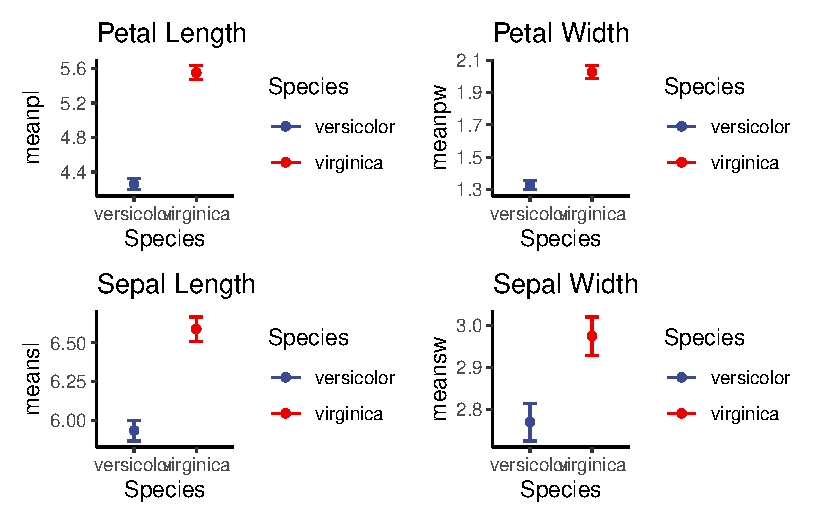
\includegraphics{cor_reg_chi_files/figure-pdf/unnamed-chunk-34-1.pdf}

}

\end{figure}

\textbf{Does Petal Length differ by species?}

\begin{Shaded}
\begin{Highlighting}[]
\NormalTok{t1}\OtherTok{\textless{}{-}}\FunctionTok{t.test}\NormalTok{(}\AttributeTok{data=}\NormalTok{iris2, Petal.Length}\SpecialCharTok{\textasciitilde{}}\NormalTok{Species, }\AttributeTok{alternative=}\StringTok{\textquotesingle{}two.sided\textquotesingle{}}\NormalTok{, }\AttributeTok{var.equal=}\ConstantTok{FALSE}\NormalTok{) }\CommentTok{\#two.sided and var.equal= FALSE are default, so we don\textquotesingle{}t have to list them. BUt, we can also change them (as I will show later)}

\NormalTok{t1 }\CommentTok{\#p\textless{}0.05 suggests that there is a significant difference in petal length between species}
\end{Highlighting}
\end{Shaded}

\begin{verbatim}

    Welch Two Sample t-test

data:  Petal.Length by Species
t = -12.604, df = 95.57, p-value < 2.2e-16
alternative hypothesis: true difference in means between group versicolor and group virginica is not equal to 0
95 percent confidence interval:
 -1.49549 -1.08851
sample estimates:
mean in group versicolor  mean in group virginica 
                   4.260                    5.552 
\end{verbatim}

\hfill\break
Our p\textless0.05 suggests that there is a significant effect of
species on petal length (petal length differs by species). BUT, do we
get a clear explanation of which group is higher or lower? Look at the
Welch T-test output and you can see the means! You can also use the
graph we made to visualize this!

\textbf{Does Petal Width differ by species?}

\begin{Shaded}
\begin{Highlighting}[]
\NormalTok{t2}\OtherTok{\textless{}{-}}\FunctionTok{t.test}\NormalTok{(}\AttributeTok{data=}\NormalTok{iris2, Petal.Width}\SpecialCharTok{\textasciitilde{}}\NormalTok{Species, }\AttributeTok{alternative=}\StringTok{\textquotesingle{}two.sided\textquotesingle{}}\NormalTok{, }\AttributeTok{var.equal=}\ConstantTok{FALSE}\NormalTok{) }\CommentTok{\#two.sided and var.equal= FALSE are default, so we don\textquotesingle{}t have to list them. BUt, we can also change them (as I will show later)}

\NormalTok{t2}
\end{Highlighting}
\end{Shaded}

\begin{verbatim}

    Welch Two Sample t-test

data:  Petal.Width by Species
t = -14.625, df = 89.043, p-value < 2.2e-16
alternative hypothesis: true difference in means between group versicolor and group virginica is not equal to 0
95 percent confidence interval:
 -0.7951002 -0.6048998
sample estimates:
mean in group versicolor  mean in group virginica 
                   1.326                    2.026 
\end{verbatim}

\hfill\break
\textbf{Does Sepal Width differ between species?}

\begin{Shaded}
\begin{Highlighting}[]
\NormalTok{t3}\OtherTok{\textless{}{-}}\FunctionTok{t.test}\NormalTok{(}\AttributeTok{data=}\NormalTok{iris2, Sepal.Width}\SpecialCharTok{\textasciitilde{}}\NormalTok{Species, }\AttributeTok{alternative=}\StringTok{\textquotesingle{}two.sided\textquotesingle{}}\NormalTok{, }\AttributeTok{var.equal=}\ConstantTok{FALSE}\NormalTok{) }\CommentTok{\#two.sided and var.equal= FALSE are default, so we don\textquotesingle{}t have to list them. BUt, we can also change them (as I will show later)}

\NormalTok{t3}
\end{Highlighting}
\end{Shaded}

\begin{verbatim}

    Welch Two Sample t-test

data:  Sepal.Width by Species
t = -3.2058, df = 97.927, p-value = 0.001819
alternative hypothesis: true difference in means between group versicolor and group virginica is not equal to 0
95 percent confidence interval:
 -0.33028364 -0.07771636
sample estimates:
mean in group versicolor  mean in group virginica 
                   2.770                    2.974 
\end{verbatim}

\hfill\break
\textbf{Does Sepal Length differ between species?}

\begin{Shaded}
\begin{Highlighting}[]
\NormalTok{t4}\OtherTok{\textless{}{-}}\FunctionTok{t.test}\NormalTok{(}\AttributeTok{data=}\NormalTok{iris2, Sepal.Length}\SpecialCharTok{\textasciitilde{}}\NormalTok{Species, }\AttributeTok{alternative=}\StringTok{\textquotesingle{}two.sided\textquotesingle{}}\NormalTok{, }\AttributeTok{var.equal=}\ConstantTok{FALSE}\NormalTok{) }\CommentTok{\#two.sided and var.equal= FALSE are default, so we don\textquotesingle{}t have to list them. BUt, we can also change them (as I will show later)}

\NormalTok{t4}
\end{Highlighting}
\end{Shaded}

\begin{verbatim}

    Welch Two Sample t-test

data:  Sepal.Length by Species
t = -5.6292, df = 94.025, p-value = 1.866e-07
alternative hypothesis: true difference in means between group versicolor and group virginica is not equal to 0
95 percent confidence interval:
 -0.8819731 -0.4220269
sample estimates:
mean in group versicolor  mean in group virginica 
                   5.936                    6.588 
\end{verbatim}

SO, when is a t-test actually useful and when isn't it? We use a T-test
\textbf{ONLY} when we want to compare two means / two populations. If we
have more than 2 groups, a T-test is not appropriate! Instead, we need
to use an analysis of variance (ANOVA) or possibly something more
complex!



\end{document}
